% main.tex - a driver for your Stata Journal insert
%
%
% The Stata Press document class
\documentclass[bib]{./sty/statapress}

% Page dimensions
\usepackage[crop,newcenter,frame]{./sty/pagedims}
% The Stata Journal styles
\usepackage{./sty/sj}
% Encapsulated PostScript figures
\usepackage{epsfig}

% Stata Log listings and useful macros
\usepackage{./sty/stata}
\usepackage{amsmath}
\usepackage{amssymb}

% Shadow package to render technical note figure
\usepackage{shadow}
% EDITORS: volume number, issue number, month, and year
\sjsetissue{$vv$}{$ii$}{$mm$}{$yyyy$}

\usepackage{threeparttable}
\usepackage{tabularx}
\usepackage{subcaption} %for subfigures
\usepackage{hyperref} %for hyperlinks. Place the package as the last to be loaded
\usepackage{algorithm}
\usepackage{algpseudocode}
\usepackage[htt]{hyphenat}

\newtheorem{remark}{Remark}
\newtheorem{suggestion}{Suggestion}
%%%%%%%%%%%%%%%%%%%%%%%%%%%%%%%%%%%%%%%%%%%%%%%%%%%%%%%%%%%%%%%%%%%%%%%%%%%%%%%%%%%%%%%%%%%%%%%%%%%%%%%%%%%%5
\begin{document}

\newcommand{\xtevent}{\texttt{xtevent }}
\newcommand{\xteventplot}{\texttt{xteventplot }}

\inserttype[st0001]{article} %in brackets the SJ article id. Below, in the keywords, it will be inserted by the \inserttag command
\author{Freyaldenhoven, Hansen, P\'erez P\'erez, Shapiro}{%
    \begin{tabular}{cc}
    Simon Freyaldenhoven & Christian B. Hansen \\
     Federal Reserve Bank of Philadelphia & University of Chicago \\
     Philadelphia, PA & Chicago, IL \\
     simon.freyaldenhoven@phil.frb.org & chansen1@chicagobooth.edu \\
     \\
    Jorge P\'erez P\'erez & Jesse M. Shapiro \\
    Banco de México & Harvard University \\
    Mexico City, Mexico & Cambridge, MA \\
    jorgepp@banxico.org.mx & jesse\_shapiro@fas.harvard.edu
    \end{tabular}
}
\title[xtevent]{xtevent: Visualization and Estimation in the Linear Panel Event-Study Design}
\maketitle

\begin{abstract}
Linear panel models, and the “event-study plots” that often accompany them, are popular tools for learning about policy effects. We introduce the \texttt{xtevent} package, which enables the construction of event-study plots following the suggestions in \cite{freyaldenhoven2021visualization}. The package implements a wide variety of popular estimators to estimate the underlying policy effects, and allows for non-binary policy variables.

\keywords{\inserttag, xtevent, xteventplot, xteventtest, get\_unit\_time\_effects, linear panel data models, two-way fixed effects regression, pre-trends, event study}
\end{abstract}

%%%%%%%%%%%% Sections %%%%%%%%%%%%%%%%%%%%%
%%%%%%%%%%%%% Section 1: introduction %%%%%%%%%%

\section{Introduction}
\label{sec:intro}
In this article, we introduce the \texttt{xtevent} package, which enables the estimation of linear panel model with dynamic policy effects under a variety of identifying assumptions. It further enables the construction of the corresponding event-study plots following the suggestions in \cite{freyaldenhoven2021visualization}.

We are interested in learning the dynamic effect of a scalar policy $z_{it}$ on some outcome $y_{it}$ in an observational panel of units $i\in\{1,...,N\}$ observed in a sequence of periods $t\in\{1,...,T\}$. We consider the following model:
\begin{align}
y_{it} =  \alpha_{i} + \gamma_{t} + q_{it}'\psi  + \sum_{m=-G}^{M}\beta_m z_{i,t-m} + C_{it} + \varepsilon_{it}. \label{eq:linear}
\end{align}
Here, $\alpha_i$ denotes a unit fixed effect, $\gamma_t$ a time fixed effect, and $q_{it}$ a vector of controls with conformable coefficients $\psi$.
The scalar $C_{it}$ denotes a (potentially unobserved) confound that may be correlated with the policy, and the scalar $\varepsilon_{it}$ represents an unobserved shock that is not correlated with the policy.
The parameters $\{\beta_{m}\}_{m=-G}^{M}$ encapsulate the dynamic effects of the policy.
Specifically, the outcome at time $t$ can be directly affected by the value of the policy at most $M \ge 0$ periods before $t$ and at most $G \geq 0 $ periods after $t$.


To visualize the dynamic treatment effect, a typical event-study plot is based on the following variation of \eqref{eq:linear} (see \citeauthor{freyaldenhoven2021visualization} \citeyear{freyaldenhoven2021visualization}):

\begin{equation}
\label{eq:event_study_plot}
    \begin{split}
        y_{it} = \sum_{k=-G-L_G}^{M+L_M -1}\delta_k \Delta  z_{i,t-k} + \delta_{M+L_M} z_{i,t-M-L_M} + \delta_{-G-L_G-1}(1-z_{i,t+G+L_G})
        \\ \centering
        + \alpha_{i} + \gamma_{t} + q'_{it}\psi + C_{it} + \varepsilon_{it},
    \end{split}
\end{equation}
where $\Delta$ denotes the first difference operator.
In \eqref{eq:event_study_plot}, the parameters $\left\{ \delta_k \right\}_{k = - G - L_G - 1}^{k = M + L_M}$ measure the cumulative effect of the policy at different horizons \citep{schmidheiny2019event}.
The corresponding event-study plot then depicts estimates of the cumulative treatment effects at different horizons $k$.
Thus, the x-axis corresponds to different values of $k$, and the y-axis corresponds to estimates of policy effects $\left\{ \hat{\delta}_k \right\}_{k = - G - L_G - 1}^{k = M + L_M}$.
We refer to $k$ as event-time, to the vector $\delta = (\delta_{-G - L_G -1}, \ldots, \delta_{M + L_M})'$ as the event-time path of the outcome, and to its estimated counterpart $\hat{\delta}$ as the estimated event-time path.

To permit the visualization of overidentifying information, \eqref{eq:event_study_plot} includes the estimated cumulative effects of the policy at horizons outside of the range of horizons over which the policy is thought to affect the outcome.
For example, it is common to rule out effects of the policy at time $t$ on the outcome in periods before $t$ ($G=0$).
By including $L_G$ additional periods in \eqref{eq:event_study_plot}, we allow a visualization of pre-event trends (``pre-trends'') that are generally inconsistent with the model in \eqref{eq:linear}.
Similarly, the estimating equation in \eqref{eq:event_study_plot} permits visualizing the estimated cumulative effect for an additional $L_M$ periods after the cumulative treatment effect is assumed to be constant in \eqref{eq:linear}.

While \eqref{eq:event_study_plot} allows for general (e.g. non binary) policy variables $z_{it}$, it is instructive to consider the special case of \textit{staggered adoption}, by which we mean that the policy is binary, all units begin without the policy; and once the policy is adopted by a given unit it is never reversed.
Then, $\Delta z_{i,t-k}$ is an indicator for whether unit $i$ adopted the policy exactly $k$ periods before period $t$,  $z_{i,t-M-L_M}$ is an indicator for whether unit $i$ adopted at least $M+L_M$ periods before period $t$, and $(1-z_{i,t+G+L_G})$ is an indicator for whether unit $i$ will adopt more than $G+L_G$ periods after period $t$.

Our package complements many other recent contributions to estimation and visualization of panel event studies in Stata. Many of these (e.g., \citep{eventddsj}; see also \citep{didmultiplegt}, \citep{didimputation}, and \citep{eventstudyinteract}) focus on the case of staggered adoption, and so by default require the user to specify a unit-specific treatment period, or to represent time relative to treatment. By contrast, our package allows for general policy variables $z_{it}$. Our package therefore allows for a default visualization in a very wide range of settings. We stress, though, that there are advantages to implementations that are designed to ensure desirable econometric properties in more specialized settings such as the one of staggered adoption. Our package incorporates one such procedure as an option.

In the following section, we briefly discuss a number of estimation strategies for \eqref{eq:event_study_plot}, provide more details on how we construct the corresponding event-study plots, and introduce some additional features included in the \xtevent package.
Then, in section \ref{sec:package}, we give a more detailed description of the syntax and options for the \texttt{xtevent} package.
In section \ref{sec:examples}, we illustrate the command in simulated data from \citet{freyaldenhoven2021visualization} and by estimating the effect of a tax reform using data from \citet{martinez2022mobility}.

%%%%%%%%%%%%%% Section 2: methods %%%%%%%%%%%%%

\section{Methods}\label{sec:methods}

\subsection{Estimation strategies}

In general, identification of the parameters $\delta$ will require some form of restriction on how observable and latent variables relate to the confound $C_{it}$ and the policy $z_{it}$.
What type of restriction is appropriate will depend on the the economic setting and can typically not be learned from the data.
In turn, the choice of restriction will determine what type of estimator is appropriate to estimate $\delta$ (see \citeauthor{freyaldenhoven2021visualization} \citeyear{freyaldenhoven2021visualization} for a more detailed discussion).
The package \texttt{xtevent} includes the following estimators.

\noindent \textbf{Two-way fixed effects estimator.}
If $C_{it} = 0$, equation \eqref{eq:event_study_plot} may be estimated by OLS using a standard two-way fixed effects estimator.
When there is only one group of fixed effects, \texttt{xtevent} uses \texttt{areg} for estimation.
\texttt{xtevent} further allows for estimation using \texttt{xtreg} or the \texttt{reghdfe} command \citep{guimaraes2010simple,Correia2017:HDFE,correia2019reghdfe} to allow for multiple or high-dimensional fixed effects.

\noindent \textbf{Controlling for unit-specific trends.}
If $C_{it} = \lambda_i f(t)$, where $f(\cdot)$ is a known low-dimensional set of basis functions (e.g. $f(t) = t$ ), then \eqref{eq:event_study_plot} may be estimated by including unit-specific time trends.
These can be included in the regression using factor variables (e.g. \texttt{i.crosssectionid\#c.time}) or absorbing them using \texttt{reghdfe}.

\noindent \textbf{Controlling for event-time trends.}
If $C_{it}$ can be written as
\begin{equation}\label{eq:trendextrapolation}
  C_{it} = \tilde{\alpha}_i + \tilde{\gamma}_t + q'_{it} \tilde{\psi} + \sum_{m} \phi' f(m) z_{i,t-m}
\end{equation}
for a known set of basis functions $f(\cdot)$ and unknown parameters $\tilde{\alpha}_i, \tilde{\gamma}_t$ and $\tilde{\psi}$, then equation \eqref{eq:event_study_plot} may be estimated by including the appropriate terms from \eqref{eq:trendextrapolation} directly in a regression model, or by GMM in a second step following estimation of \eqref{eq:event_study_plot}  via two-way fixed effects.

Intuitively, if the confound can be approximated by a trend in event-time, then we can learn about the trend in periods where the policy is inactive (i.e., $k<0$) and extrapolate it to later periods.
The differences between the outcome variable and the extrapolated trend are then informative of the policy effects \citep{dobkin2018economic}.
As a specific example, consider a staggered adoption setting where the confound follows a linear trend in time, this trend starts 3 periods before the policy activates, and continues for 3 periods afterwards.
We can represent this situation by taking $f(m) = 1$ if $m \in \left[-3,3\right]$ and $f(m)=0$ otherwise. In this case, we can extrapolate the trend to post-adoption periods and subtract it to account for the confound.

We allow $z_{it}$ to be continuous and adoption may not be staggered.
If equation \eqref{eq:trendextrapolation} holds, then the estimand of a standard two-way fixed effect estimator of equation \eqref{eq:trendextrapolation} is given by
\begin{equation}\label{eq:trendcases}
  d_k =
  \begin{cases}
    \phi' f_k, & \mbox{if } k < -G \\
    \delta_k + \phi' f_k, & \mbox{if } -G \leq k \leq M \\
    \delta_M + \phi'f_k, & \mbox{otherwise},
  \end{cases}
\end{equation}
where $f_k = \sum_{m = -\infty}^{k} f(m)$.

Given estimates of $d_k$, $\hat{d_k}$, we can recover the trend parameters $\phi$ from the estimates $\hat{d}_k$ in the $L_G$ unaffected periods.
Let $T_G \leq L_G$ be the number of periods prior to $G$ used estimate the trend parameters, and $T_M \leq M$ be the number of ``post-event'' periods where the trend is active.
We assume $f_k \neq 0$ for $k \in \left[-G-T_G,T_M \right]$ and $0$ otherwise.
We can recover the trend parameters by using the $T_G$ moment conditions $\hat{d}_k - \phi' f_k = 0$ for $k = -G - T_G,\ldots,-G-1$.
We can then calculate an adjusted event-time path $\hat{\delta}$ that accounts for the confound by subtracting $\phi f_k$ from the unadjusted coefficients $d_k$ for $k \in \left[-G-T_G,T_M\right]$.
Appendix \ref{sec:app_trend} provides further details about this estimator.

\noindent \textbf{IV estimation with multiple proxies.}
If multiple additional variables are available that may serve as proxies for the confound $C_{it}$, such that

\begin{equation}\label{eq:proxy}
  x_{it} = \alpha_i^x + \gamma_t^x + \phi^x q_{it} + \Xi^x \eta_{it} + u_{it}
\end{equation}
with unknown parameters $\alpha_i^x, \gamma_t^x, \Xi^x$ and an unobserved vector $u_{it}$ (which is uncorrelated across proxies), then equation \eqref{eq:event_study_plot} may be estimated by including one of the proxies in \eqref{eq:event_study_plot} and instrumenting for it using the other proxy variable.

\noindent \textbf{IV estimation with single proxy.}
If only a single additional variable is available that may serve as proxy for the confound $C_{it}$, with the error in equation \eqref{eq:proxy} conditionally mean-independent of the policy, then equation \eqref{eq:event_study_plot} may be estimated using a two-stage least squares estimator, instrumenting for the proxy with leads of the policy variable \citep{freyaldenhoven2019pre}.

In principle, all leads of the policy variable further out than $G$ are potential instruments.
To choose among these, we estimate \eqref{eq:event_study_plot} via two-way fixed effects, with the proxy as the outcome variable.
We then choose among the leads $\{\Delta z_{i,t+k}\}_{k=G+1}^{G+L_G}$ and $z_{i,t+G+L_G}$ the one with the largest absolute t-statistic to serve as the default excluded instrument for estimation of \eqref{eq:event_study_plot}.

%If the proxy is conditionally mean-independent of the policy, and if there is a correlation between the outcome variable and the proxy in the pre-event periods, this relationship must be mediated by the confound. The pre-trends in the proxy and the outcome can then be used to estimate the effect of the confound on the outcome variable. \cite{freyaldenhoven2019pre} show that in this setting, we can estimate $\delta$ by including the proxy in \eqref{eq:event_study_plot} and instrumenting it with leads of the policy.%Their approach requires that the noise in the proxy is conditionally mean-independent of the policy.

\subsection{Event-Study Plots}
\label{subsec:plots}

The auxiliary command \texttt{xteventplot} includes functionality to visualize the event-study plots based on any of the estimators from the previous section.
It further includes the enhancements to these plots suggested in \cite{freyaldenhoven2021visualization}.

\noindent \textbf{Normalization.}
Because the policy variables in \eqref{eq:event_study_plot} are collinear, a normalization is required to identify the event-time path $\left\{ \delta_k \right\}_{k = - G - L_G - 1}^{k = M + L_M}$.
\texttt{xtevent} normalizes $\delta_{-1}=0$ by default. In the case of staggered adoption this normalization implies that  the plotted coefficients can be interpreted as estimated effects relative to the period before the policy is enacted.

\noindent \textbf{Outcome variable level.}
To ease interpretation of the estimated policy effects, \xtevent includes a parenthetical label for the normalized coefficient that reflects the mean of the dependent variable.
For instance, in the case of staggered adoption, under our default normalization the label corresponds to the sample mean of $y_{it}$ one period before adoption.
More generally, the label corresponds to the value $$\frac{\sum_{(i,t): \Delta z_{i,t-k^{\star}} \neq 0} y_{it}}{ \left| (i,t) : \Delta z_{i,t-k^{\star}} \neq 0 \right| }$$ where $\delta_{k^{\star}}$ is the normalized cofficient.

\begin{sloppypar}
\noindent \textbf{Uniform inference.}
In addition to standard pointwise confidence intervals for the coefficients $\delta_k$, \xtevent allows for plotting of uniform sup-t confidence bands \citep{freyberger2018uniform,montiel2019simultaneous}.
The inclusion of these bands allows for visual tests of hypotheses about the entire coefficient path instead of just single coefficients.
\end{sloppypar}

\noindent \textbf{Overidentification and testing.}
The estimating equation in \eqref{eq:event_study_plot} includes $L_G$ additional periods before the policy is enacted to visualize potential pre-trends.
Evidence of such pre-trends is in practice often seen as evidence for the presence of a confound that invalidates the research design.
The estimating equation in \eqref{eq:event_study_plot} also includes $L_M$ additional periods after the policy effects end to assess if the dynamic effects have leveled off after the $M$ postulated periods for which the policy has a direct effect.
\xtevent displays the p-values of Wald tests for ``pre-trends'' ($\delta_k = 0 \text{ for } -G - L_G - 1 \leq k < -G$) and for dynamic effects ``leveling-off'' ($ \delta_M =\delta_{M+k} \text{ for } 0 < k \leq L_M$).
The auxiliary command \texttt{xteventtest} allows for testing additional hypotheses, such as hypotheses about cumulative effects, about whether effects are constant, and about whether the effects follow linear trends.

\noindent \textbf{Least wiggly path of confounds consistent with the estimates.} %Neither visual absence of pretrends or failure to reject the null of no pre-trends imply the absence of a confound.
To help visualize whether there exists a confound that can plausibly explain all of the event time dynamics of the outcome variable, \xtevent allows for adding a representation of the ``most plausible'' confound trajectory that is consistent with the absence of policy effects.
Our choice of ``most plausible'' confound is the least ``wiggly'' polynomial in event-time that passes through the Wald confidence region of the event-time path.
The idea is that, if a ``smooth'' path exists, this suggests that a confound could plausibly explain the entire event time path of the outcome, even absent any policy effects.
On the other hand, if no ``smooth'' path exists, this may be indicative that a confound cannot plausibly explain the entire event-time path of the outcome, and therefore that the policy does affect the outcome.
We describe the computation of the least wiggly path in detail in Appendix \ref{sec:smoothest_path}.

\noindent \textbf{Overlay plots.}
\xteventplot allows event-study plots with overlays in different estimation scenarios. For estimation with event-time trends, \xteventplot creates plots overlaying the event-time trend.
For IV estimation with proxies, \xteventplot allows overlaying the dynamics implied by the proxy variable.
\xteventplot also allows overlays of a constant-effects model to visually assess if the policy effects are constant over time.


\subsection{Additional features}

The package includes the following additional capabilities.

\noindent \textbf{Imputation of missing values in the policy variable.}
Because equation \eqref{eq:linear} includes leads and lags of the policy variable $z_{it}$ and its first difference, the estimation sample may be smaller than the entire sample available.
In general, if the outcome variable is observed for $t \in \left\{\underline{t},\ldots,\overline{t} \right\}$, we need to observe the policy variable $z_{it}$ from $\underline{t} - G - L_G$ to $\overline{t} + M + L_M -1$ to avoid dropping observations from the estimation sample.
In a typical setup, this may imply that we need to restrict the estimation window in order to calculate the necessary leads and lags of $z_{it}$.
However, the user may have additional information that allows imputation of the policy variable.

\xtevent allows for the following imputation schemes:
\begin{enumerate}
\item If the policy variable is declared to follow staggered adoption, \xtevent can:
\begin{enumerate}
\item automatically impute any missing values in the policy variable \textit{outside} the observed data range assuming no policy changes outside the sample period.
For example, if we observe $z_{jt}=1$, under staggered adoption this implies that $z_{js}=1$ for $s>t$.
\item automatically impute missing values of the policy variable \textit{inside} the observed data range. For example, if $z_{jt} = 1$ and $z_{j,t+2} = 1$, this implies that $z_{j,t+1} = 1$.
\end{enumerate}
\item
Even absent staggered adoption, if the policy variable is declared not to change values outside the observed sample, \xtevent can automatically impute $z_{it}$ outside of the observed sample.
For example, if the sample starts at $\underline{t}$ and $z_{1\underline{t}} = 0$ for unit 1, we set $z_{it} = 0$ for $t \in \{ \underline{t} - G - L_G, ..., \underline{t}-1 \}$.
\end{enumerate}

\noindent \textbf{Estimation with repeated cross-sectional data}. Some setups involve repeated cross sectional data instead of panel data with treatment varying at a higher level of aggregation. For example, we may have a series of repeated cross-sections of individuals for each US state $s$ and a state-level policy $z_{st}$. In this environment, estimating \eqref{eq:event_study_plot} with individual fixed effects is unfeasible, but \xtevent allows estimation of a related model with fixed effects by state:
\begin{equation}\label{eq:repeatedcs}
    \begin{split}
        y_{it} = \sum_{k=-G-l_G}^{M+L_M -1}\delta_k \Delta  z_{s(i),t-k} + \delta_{M+L_M} z_{s(i),t-M-L_M} + \delta_{-G-L_G-1}(1-z_{s(i),t+G+L_G})
        \\ \centering
        + \alpha_{s(i)} + \gamma_{t} + q'_{it}\psi + C_{s(i)t} + \varepsilon_{it},
    \end{split}
\end{equation}
where the parameters $\alpha_{s(i)}$ are fixed effects corresponding to state $s$ where unit $i$ belongs.

An alternative \citep{amemiya1978note, hansen2007generalized} is to regress $y_{it}$ on a set of state-time indicators, plus any control variables $q_{it}$ that vary at the individual level, and then estimate \eqref{eq:event_study_plot} with the estimated state-time effects as dependent variables, and including state fixed effects, time fixed effects, and controls that vary at the state level.
The auxiliary command \texttt{get\_unit\_time\_effects} facilitates this approach.

\textbf{Heterogenous treatment effects in staggered adoption settings.} The model in equation \eqref{eq:linear} assumes that the causal effect of the policy is homogeneous over units $i$.
A recent literature has highlighted that if treatment effects are heterogeneous by treatment time, then the effects estimated with equation \eqref{eq:linear} may not be properly-weighted averages of the cohort-level treatment effects \citep{athey2022design,callaway2021difference,goodman2021difference,sun2021estimating}.
\cite{sun2021estimating} propose to estimate event studies for each treated cohort separately, comparing each one to an untreated cohort, and then averaging the effects weighting by the percentage of treated units in each cohort, to arrive at a treatment effect on the treated.
For the two-way fixed effects case, and under staggered adoption, \texttt{xtevent} allows for estimation of cohort-by-cohort estimates, in which case it reports an average weighted by the number of treated observations in each cohort, which is an estimate of a weighted average treatment effect on the treated.

%%%%%%%%%%%%%% Section 3: about the xtevent package %%%%%%%%%%%%%

\section{The xtevent package}\label{sec:package}
The xtevent package includes the commands \texttt{xtevent} for estimation, \texttt{xteventplot} for visualization, and \texttt{xteventtest} for postestimation hypothesis testing. It also includes \texttt{get\_unit\_time\_effects}, an auxiliary command to be used in combination with \texttt{xtevent} in repeated cross-section settings. This section describes the syntax and options of each of these commands.

%%%%%%%%%%%%%%%%%

\subsection{The xtevent command}
The \texttt{xtevent} command has the following syntax:

\begin{stsyntax}
xtevent
    \depvar\
    \optindepvars\
    \optif\
    \optin\
    \optweight\
    \emph{,}
    \texttt{\underbar{pol}icyvar(\varname)}
    \texttt{\underbar{p}anelvar(\varname)}\
    \texttt{\underbar{t}imevar(\varname)}\
    \optional{\it options}

\end{stsyntax}




\subsubsection{Options}
\hangpara
\texttt{policyvar(\varname)} specifies the policy variable of interest. \texttt{policyvar()} is required.

\hangpara
\texttt{panelvar(\varname)} specifies the cross-sectional identifier variable that identifies the panels.
\texttt{panelvar()} is required if the data have not been  previously \texttt{xtset}.

\hangpara
\texttt{timevar(\varname)} specifies the time variable. \texttt{timevar()} is required if the data have not been previously \texttt{xtset}.

\hangpara
{\tt window({\it numlist})} specifies the window around the policy change event to estimate dynamic effects. If a single positive integer $k>0$ is specified, the estimation will use a symmetric window of $k$ periods around the event.
For example, if $k = 2$, there will be five coefficients in the window $\{-2,-1,0,1,2\}$ and two endpoints $\{-3+, 3+\}$.
If two distinct integers, $k_1\le0$ and $k_2\ge0$, are specified, the estimation will use an asymmetric window with $k_1$ periods before the event and $k_2$ periods after the event.
For example, with $k_1 = -1$ and $k_2 = 2$, there will be four coefficients in the window $\{-1,0,1,2\}$ and two endpoints $\{-2+,3+\}$.
{\tt window()} is required unless {\tt static} is specified, or if the estimation window is specified using options {\tt pre(), post(), overidpre()} and {\tt overidpost()} (See below).

\hangpara
{\tt pre, post, overidpre} and {\tt overidpost} offer an alternative way to specify the estimation window:

\morehangpara
{\tt pre} is the number of pre-event periods where anticipation effects are allowed.
With {\tt window}, {\tt pre} is 0.

\morehangpara
{\tt post} is the number of post-event periods where policy effects are allowed.
With {\tt window}, {\tt post} is the number of periods after the event (not including the period for the event, e.g. event time = 0).

\morehangpara
{\tt overidpre} is the number of pre-event periods for an overidentification test of pre-trends. With {\tt window}, {\tt overidpre} is the number of periods before the event.

\morehangpara
{\tt overidpost} is the number of post-event periods for an overidentification test of effects leveling off. With {\tt window}, {\tt overidpost} is 1.

\hangpara
Only one of {\tt window} or {\tt pre, post, overidpre} and {\tt overidpost} can be declared.

\hangpara
{\tt norm({\it integer})} specifies the event-time coefficient to be normalized to 0. The default is to normalize the coefficient on -1.

\hangpara
{\tt proxy({\it varlist})} specifies proxy variables for the confound to be included.

\hangpara
{\tt proxyiv({\it string})} specifies instruments for the proxy variable for the policy.
{\tt proxyiv()} admits three syntaxes to use either leads of the policy variable or additional variables as instruments.
The default is to use leads of the difference of the policy variable as instruments, selecting the lead with the strongest first stage.

\morehangpara
{\tt proxyiv(select)} selects the lead with the strongest first stage among all possible leads of the differenced policy variable to be used as an instrument.
{\tt proxyiv(select)} is the default for the one proxy, one instrument case, and it is only available in this case.

\morehangpara
{\tt proxyiv(\# ...)} specifies a numlist with the leads of the differenced policy variable as instruments. For example, {\tt proxyiv(1 2)} specifies that the two first leads of the difference of the policy variable will be used as instruments.

\morehangpara
{\tt proxyiv({\it varlist})} specifies a \textit{varlist} with the additional variables to be used as instruments.

\hangpara
{\tt nofe} excludes panel fixed effects.

\hangpara
{\tt note} excludes time fixed effects.

\hangpara
{\tt impute({\it type}, [{\it saveimp}]) }imputes missing values in {\it policyvar} and uses this new variable as the actual {\it policyvar}. {\tt type} determines the imputation rule. The suboption {\tt saveimp} adds the new variable to the database as {\it policyvar\_imputed}. The following imputation types can be implemented:

\morehangpara
{\tt impute(nuchange)} imputes missing values in {\it policyvar} according to {\it no-unobserved change}: it assumes that, for each unit: i) in periods before the first observed value, the policy value is the same as the first observed value and; ii) in periods after the last observed value, the policy value is the same as the last observed value.

\morehangpara
{\tt impute(stag)} applies {\it no-unobserved change} if {\it policyvar} satisfies staggered-adoption assumptions for all units: i) {\it policyvar} must be binary; and ii) once {\it policyvar} reaches the adopted-policy state, it never reverts to the unadopted-policy state. See \citet{freyaldenhoven2021visualization} for detailed explanation of the staggered adoption case.

\morehangpara
{\tt impute(instag)} applies {\tt impute(stag)} and additionally imputes missing values inside the observed data range: a missing value or a group of them will be imputed only if they are both preceded and followed by the unadopted-policy state or by the adopted-policy state.

\hangpara
{\tt static} estimates a static panel data model and does not generate or plot event-time dummies.
{\tt static} is not allowed with {\tt window}, {\tt pre}, {\tt post}, {\tt overidpre}, {\tt overidpost}, or {\tt diffavg}.

\hangpara
{\tt diffavg} calculates the difference in averages between the post-event estimated coefficients and the pre-event estimated coefficients periods.
It also calculates its standard error with {\tt lincom}. {\tt diffavg} is not allowed with {\tt static}.

\hangpara
{\tt trend({\it \#1} [,{\it subopt}])} extrapolates a linear trend using the time periods from period {\it \#1} before the policy change to one period before the policy change, as in \citet{dobkin2018economic}.
For example, {\tt trend(-3)} uses the coefficients on event-times -3, -2, and -1 to estimate the trend.
The estimated effect of the policy is the deviation from the extrapolated linear trend.
{\it \#1} must be less than {\it -1}.
{\tt trend} is only available when the normalized coefficient is -1 and {\it pre} = 0.
The following can be passed as suboptions:

\morehangpara
{\tt method({\it string})} sets the method to estimate the linear trend. It can be Ordinary Least Squares ({\it ols}) or Generalized Method of Moments ({\it gmm}). ({\it ols}) omits the event-time dummies from trend({\it \#1}) to {\it -1} and adds a linear trend ({\it \_ttrend}) to the regression. ({\it gmm}) uses the GMM to compute the trend for the event-time dummy coefficients. The default is {\tt method({\it gmm})}.

\morehangpara
{\tt saveoverlay} saves estimations for the overlay plot produced by
            {\tt xteventplot, overlay({\it trend})}.

\hangpara
{\tt savek({\it stub})} saves variables for time-to-event, event-time, trend, and interaction variables.
Event-time dummies are stored as {\it stub\_eq\_m\#} for the dummy variable {\it \#} periods before the policy change, and {\it stub\_p\#} for the dummy variable {\it \#} periods after the policy change.
The dummy variable for the policy change time is {\it stub\_p0}
 Event time is stored as {\it stub\_evtime}. The trend is stored as {\it stub\_trend}.
For estimation with the \citet{sun2021estimating} method, such that {\tt cohort} and {\tt control\_cohort} are active, the interaction variables are stored as {\it stub\_m\#\_c\#} or {\it stub\_p\#\_c\#}, where {\it c\#} indicates the cohort.
The following suboptions can be specified:

\morehangpara
{\tt noestimate} saves variables for event-time dummies, event-time and trends without estimating the model. This is useful if the users want to customize their regressions and plots.

\morehangpara
{\tt saveinteract} saves interaction variables if {\tt cohort} and {\tt control\_cohort} are specified. {\tt noestimate} and {\tt saveinteract} cannot be specified simultaneously.

\hangpara
{\tt usek({\it stub})} uses previously used event-time dummies saved with prefix {\it stub}. This can be used to speed up estimation.

\hangpara
{\tt reghdfe} uses reghdfe for estimation, instead of {\tt areg, ivregress and  xtivreg}.
{\tt reghdfe} is useful for large datasets.
By default, it absorbs the panel fixed effects and the time fixed effects.
For OLS estimation, the {\tt reghdfe} option requires {\tt reghdfe} and {\tt ftools} to be installed. For IV estimation, it also requires {\tt ivreghdfe} and {\tt ivreg2} to be installed.
Note that standard errors may be different and singleton clusters may be dropped using {\tt reghdfe}.
See \citet{Correia2017:HDFE}.

\hangpara
{\tt addabsorb({\it varlist})} specifies additional fixed effects to be absorbed when using {\tt reghdfe}.
By default, {\tt xtevent} includes time and unit fixed effects.
{\tt addabsorb} requires {\tt reghdfe}.

\hangpara
{\tt repeatedcs} indicates that the dataset in memory is repeated cross-sectional.
In this case, {\tt panelvar} should indicate the groups at which {\tt policyvar} changes.
For instance, {\tt panelvar} could indicate states at which {\tt policyvar} changes, while the observations in the dataset are individuals in each state.
There is an alternative method to estimate the event study in a repeated cross-sectional dataset, which involves using {\tt  get\_unit\_time\_effects} first, and then {\tt xtevent}.
See the description of the {\tt get\_unit\_time\_effects} command below.
For fixed-effects estimation, {\tt repeatedcs} enables {\tt reghdfe}.

\hangpara
{\tt cohort({\it varname})} specifies the variable that identifies the cohort for each unit.
{\tt cohort} and {\tt control\_cohort} indicate {\tt xtevent} to estimate the event-time coefficients with the estimator of \citet{sun2021estimating} for settings with heterogeneous effects by cohort.
{\tt cohort} requires the Stata module {\tt avar}.

\hangpara
{\tt control\_cohort({\it varname})} specifies the binary variable that identifies the control cohort. {\tt cohort} and {\tt control\_cohort} indicate {\tt xtevent} to estimate the event-time coefficients with the estimator of \citet{sun2021estimating} for settings with heterogeneous effects by cohort.
{\tt control\_cohort} requires the Stata module {\tt avar}.

\hangpara
{\tt plot} displays a default event study plot with 95\% and sup-t confidence intervals. See \citet{montiel2019simultaneous}.  Additional options are available with the postestimation command {\tt xteventplot}.

\hangpara
{\it additional\_options}: Additional options to be passed to the estimation command.
When {\tt proxy} is specified, these options are passed to {\tt ivregress}.
When {\tt reghdfe} is specified, these options are passed to {\tt reghdfe}.
Otherwise, they are passed to {\tt areg} or to {\tt regress} if {\tt nofe} is specified.
This is useful to calculate clustered standard errors or to change regression reporting.
Note that two-way clustering is allowed with {\tt reghdfe}.

\subsubsection{Saved Results}
{\tt xtevent} saves the following in {\tt e()}:

\begin{stresults2}
\stresultsgroup{Scalars} \\
\stcmd{e(lwindow)} & left endpoint for estimation window
\\
\stcmd{e(rwindow)} & right endpoint for estimation window
\\
\stresultsgroup{Macros} \\
\stcmd{e(names)} & names of the variables for the event-time dummies
\\
\stcmd{e(y1)} & mean of dependent variable et event-time = -1
\\
\stcmd{e(x1)} & mean of proxy variable at event-time = -1, when only one proxy is specified
\\
\stcmd{e(trend)} & ``trend" if estimation included extrapolation of a linear trend
\\
\stcmd{e(cmd)} & estimation command: can be regress, areg, ivregress, xtivreg, or reghdfe
\\
\stcmd{e(df)} & degrees of freedom
\\
\stcmd{e(komit)} & list of lags/leads omitted from regression
\\
\stcmd{e(kmiss)} & list of lags/leads to be omitted from plot
\\
\stcmd{e(method)} & ``ols" or ``iv"
\\
\stcmd{e(cmd2)} & ``xtevent"
\\
\stcmd{e(depvar)} & dependent variable
\\
\stcmd{e(pre)} & number of periods with anticipation effects
\\
\stcmd{e(post)} & number of periods with policy effects
\\
\stcmd{e(overidpre)} & number of periods to test for pre-trends
\\
\stcmd{e(overidpost)} & number of periods to test for effects leveling off
\\
\stcmd{e(stub)} & prefix for saved event-time dummy variables
\\
\stresultsgroup{Matrices} \\
\stcmd{e(b)} & coefficient vector
\\
\stcmd{e(V)} & variance--covariance matrix
\\
\stcmd{e(delta)} & coefficient vector of event-time dummies
\\
\stcmd{e(Vdelta)} & variance-covariance matrix of the event-time dummies coefficients
\\
\stcmd{e(deltax)} & coefficients for proxy event study to be used in overlay plot
\\
\stcmd{e(deltaxsc)} & scaled coefficients for proxy event study to be used in overlay plot
\\
\stcmd{e(deltaov)} & coefficients for event study to be used in overlay plot
\\
\stcmd{e(Vdeltax)} & variance-covariance matrix of proxy event study coefficients for overlay plot
\\
\stcmd{e(Vdeltaov)} & variance-covariance matrix of event study coefficients for overlay plot
\\
\stcmd{e(mattrendy)} & matrix with y-axis values of trend for overlay plot, only when \stcmd{ trend(\#1)} is specified
\\
\stcmd{e(mattrendx)} & matrix with x-axis values of trend for overlay plot, only when \stcmd{ trend(\#1)} is specified
\\
\stcmd{e(Sigma\_ff)} & variance estimate of the cohort share estimators, only when \stcmd{cohort} and \stcmd{control\_cohort} are specified
\\
\stcmd{e(ff\_w)} & each column vector contains estimates of cohort shares underlying the given relative time, only when \stcmd{cohort} and \stcmd{control\_cohort} are specified
\\
\stcmd{e(V\_interact)} & each column vector contains variance estimate of the cohort-specific effect estimator for the given relative time, only when \stcmd{cohort} and \stcmd{control\_cohort} are specified
\\
\stcmd{e(b\_interact)} & each column vector contains estimates of cohort-specific effect for the given relative time, only when \stcmd{cohort} and \stcmd{control\_cohort} are specified
\\
\stresultsgroup{Functions} \\
\stcmd{e(sample)} & marks estimation sample
\\
\end{stresults2}

%%%%%%%%%%%%%%%%%
\subsection{The xteventplot command}
The \texttt{xteventplot} command produces event-study plots after \texttt{xtevent}. The syntax is the following:
\begin{stsyntax}
xteventplot ,
\optional{\it options}
\end{stsyntax}

\subsubsection{Options}
\hangpara
\sloppypar \noindent
\texttt{suptreps({\it integer})} specifies the number of repetitions to calculate \citet{montiel2019simultaneous} sup-t confidence intervals for the dynamic effects. The default is 10000.


\hangpara
\texttt{overlay({\it string})} creates overlay plots for trend extrapolation, instrumental variables estimation in presence of pre-trends, and constant policy effects over time.

\morehangpara
\texttt{overlay(trend)} overlays the event-time coefficients for the trajectory of the dependent variable and the extrapolated linear trend.
\texttt{overlay(trend)} is only available after \texttt{xtevent, trend(,saveoverlay)}.

\morehangpara
\texttt{overlay(iv)} overlays the event-time coefficients trajectory of the dependent variable and the proxy variable used to infer the trend of the confounder.
\texttt{overlay(iv)} is only available after \texttt{xtevent, proxy() proxyiv()}.

\morehangpara
\texttt{overlay(static)} overlays the event-time coefficients from the estimated model and the coefficients implied by a constant policy effect over time.
These coefficients are calculated by
(i) estimating a model where the policy affects the outcome contemporaneously and its effect is constant,
(ii) obtaining predicted values of the outcome variable from this constant effects model, and
(iii) regressing the predicted values on event-time dummy variables.

\hangpara
\texttt{y} creates an event-study plot of the dependent variable in instrumental variables estimation.
\texttt{y} is only available after \texttt{xtevent, proxy() proxyiv()}.

\hangpara
\texttt{proxy} creates an event-study plot of the proxy variable in instrumental variables estimation.
\texttt{proxy} is only available after \texttt{xtevent, proxy() proxyiv()}.

\hangpara
\texttt{levels({\it numlist})} customizes the confidence level for the confidence intervals in the event-study plot.
By default, two confidence intervals -- a standard confidence interval and a sup-t confidence interval --  are drawn.
\texttt{levels} allows different confidence levels for standard confidence intervals.
For example, \texttt{levels({\it 90 95})} draws both 90\% and 95\% level confidence intervals, along with a sup-t confidence interval for Stata's default confidence level.

\hangpara
\texttt{smpath([{\it type , subopt}])} displays the ``least wiggly`` path through the Wald confidence region of the event-time coefficients.
\texttt{type} determines the line type, which may be \texttt{scatter} or \texttt{line}.
\texttt{smpath} is not allowed with \texttt{noci}.

\hangpara
The following suboptions for \texttt{smpath} control the optimization process. Because of the nature of the optimization problem, optimization error messages 4 and 5 (missing derivatives) or 8 (flat regions) may be frequent. Nevertheless, the approximate results from the optimization should be close to the results that would be obtained with convergence of the optimization process. Modifying these optimization suboptions may improve optimization behavior.

\morehangpara
\texttt{postwindow({\it scalar $>$ 0})} sets the number of post event coefficient estimates to use for calculating the smoothest line. The default is to use all the estimates in the post event window.

\morehangpara
\texttt{maxiter({\it integer})} sets the maximum number of inner iterations for optimization. The default is 100.

\morehangpara
\texttt{maxorder({\it integer})} sets the maximum order for the polynomial smoothest line. \texttt{maxorder} must be between 1 and 10. The default is 10.

\morehangpara
\texttt{technique({\it string})} sets the optimization technique for the inner iterations of the quadratic program.  ``nr", ``bfgs", ``dfp", and combinations are allowed. See maximize. The default is ``nr 5 bfgs".

\hangpara
\texttt{overidpre} changes the coefficients to be tested for the pre-trends overidentification test.
The default is to test all pre-event coefficients.
\texttt{overidpre({\it \#1})} tests if the coefficients for the earliest {\it \#1} periods before the event are equal to {\it 0}, including the endpoints.
For example, with a window of 3, \texttt{overidpre(2)} tests that the coefficients for event-times -4+ (the endpoint) and -3 are jointly equal to 0.
{\it \#1} must be greater than {\it 0}.
See the \texttt{xteventtest} command below.

\hangpara
\texttt{overidpost} changes the coefficients to be tested for the leveling-off overidentification test.
The default is to test that the rightmost coefficient and the previous coefficient are equal.
\texttt{overidpost({\it \#1})} tests if the coefficients for the latest {\it \#1} periods after the event are equal to each other, including the endpoints.
For example, with a window of 3, \texttt{overidpost(3)} tests that the coefficients for event-times 4+ (the endpoint), 3, and 2 are equal to each other.
{\it \#1} must be greater than {\it 1}.
See the \texttt{xteventtest} command below.

\hangpara
The following options control the appearance of the plot:

\hangpara
\texttt{noci} omits the display and calculation of both Wald and sup-t confidence intervals. \texttt{noci} overrides \texttt{suptreps} if it is specified.  \texttt{noci} is not allowed with \texttt{smpath}.

\hangpara
\texttt{nosupt} omits the display and calculation of sup-t confidence intervals. \texttt{nosupt} overrides \texttt{suptreps} if it is specified.

\hangpara
\texttt{nozeroline} omits the display of the reference line at {\it 0}. Note that reference lines with different styles can be obtained by removing the default line with \texttt{nozeroline} and adding other lines with \texttt{yline}. See \texttt{added\_line\_options}.

\hangpara
\texttt{nonormlabel} suppresses the vertical-axis label for the mean of the dependent variable at event-time corresponding to the normalized coefficient.

\hangpara
\texttt{noprepval} omits the display of the p-value for a test for pre-trends.
By default, this is a Wald test for all the pre-event coefficients being equal to $0$, unless \texttt{overidpre} is specified.

\hangpara
\texttt{nopostpval} omits the display of the p-value for a test for effects leveling off.
By default, this is a Wald test for the last post-event coefficients being equal, unless \texttt{overidpost} is specified.

\hangpara
\texttt{scatterplotopts} specifies options to be passed to \texttt{scatter} for the coefficients' plot.

\hangpara
\texttt{ciplotopts} specifies options to be passed to \texttt{rcap} for the confidence interval's plot.
These options are disabled if \texttt{noci} is specified.

\hangpara
\texttt{suptciplotopts} specifies options to be passed to \texttt{rcap} for the sup-t confidence interval plot.
These options are disabled if \texttt{nosupt} is specified.

\hangpara
\texttt{smplotopts} specifies options to be passed to \texttt{line} for the smoothest path through the confidence region plot.
These options are only active if \texttt{smpath} is specified.

\hangpara
\texttt{trendplotopts} specifies options to be passed to \texttt{line} for the extrapolated trend overlay plot.
These options are only active if \texttt{overlay({\it trend})} is specified.

\hangpara
\texttt{staticovplotopts} specifies options to be passed to \texttt{line} for the static effect overlay plot.
These options are only active if \texttt{overlay({\it static})} is specified.

\hangpara
\texttt{addplots} specifies additional plots to be overlaid to the event-study plot.

\hangpara
\texttt{textboxoption} specifies options to be passed to the textbox of the pre-trend and leveling-off tests.
These options are disabled if \texttt{noprepval} and \texttt{nopostval} are specified.
See \texttt{textbox\_options}.

\hangpara
{\it additional\_options}: Additional options to be passed to \texttt{twoway}.
See \texttt{twoway}.

%%%%%%%%%%%%%%%%%
\subsection{The xteventtest command}
The \texttt{xteventtest} command performs hypothesis testing after the \texttt{xtevent} command. The syntax is the following:

\begin{stsyntax}
xteventtest ,
\optional{\it options}
\end{stsyntax}

\subsubsection{Options}
\hangpara
\texttt{coefs({\it numlist})} specifies a numeric list of event-times to be tested. These are tested to be equal to $0$ jointly, unless otherwise requested in \texttt{testopts()}.

\hangpara
\texttt{cumul} requests a test of equality to $0$ for the sum of every coefficient for each event-time in \texttt{coefs()}.

\hangpara
\texttt{allpre} tests that all pre-event coefficients are equal to $0$. With \texttt{cumul}, it tests that the sum of all pre-event coefficients is equal to $0$.

\hangpara
\texttt{allpost} tests that all post-event coefficients are equal to $0$. With \texttt{cumul}, it tests that the sum of all post-event coefficients is equal to $0$.

\hangpara
\texttt{linpretrend} requests a specification test to see if the coefficients before the event follow a linear trend.

\hangpara
\texttt{trend({\it \#1})} tests for a linear trend from time period {\it \#1} before the policy change. It uses \texttt{xtevent, trend({\it \#1, method(ols)})} to estimate the trend. {\it \#1} must be less than $0$.

\hangpara
\texttt{constanteff} tests that all post-event coefficients are equal.

\hangpara
\texttt{overid} tests overidentifying restrictions: a test for pre-trends and a test for events leveling-off. The periods to be tested are those used in the \texttt{xtevent} call. See xtevent.

\hangpara
\texttt{overidpre({\it \#1})} tests the pre-trends overidentifying restriction. It tests that the coefficients for the earliest {\it \#1} periods before the event are equal to $0$, including the endpoints.
For example, with a window of 3, \texttt{overidpre(2)} tests that the coefficients for event-times -4+ (the endpoint) and -3 are jointly equal to 0.
{\it \#1} must be greater than $0$.

\hangpara
\texttt{overidpost({\it \#1})} tests the effects leveling off overidentifying restriction. It tests that the coefficients for the latest {\it \#1} periods after the event are equal, including the endpoints.
For example, with a window of 3, \texttt{overidpost(3)} tests that the coefficients for event-times 4+ (the endpoint), 3, and 2 are equal to each other.
{\it \#1} must be greater than $1$.

\hangpara
\texttt{testopts({\it string})} specifies options to be passed to \texttt{test}. See \texttt{test}.


\subsubsection{Saved Results}
{\tt xteventtest} stores the following in {\tt r()}:


\begin{stresults2}
\stresultsgroup{Scalars} \\
\stcmd{r(p)} & two-sided p-value
\\
\stcmd{r(F)} & $\scriptstyle F$ statistic
\\
\stcmd{r(df)} & test constraints degrees of freedom
\\
\stcmd{r(df\_r)} & residual degrees of freedom
\\
\stcmd{r(dropped\_i)} & index of ith constraint dropped
\\
\stcmd{r(chi2)} & chi-squared
\\
\stcmd{r(drop))} & {\it 1} if constraints were dropped, {\it 0} otherwise
\\
\stresultsgroup{Macros} \\
\stcmd{r(mtmethod)} & method of adjustment for multiple testing
\\
\stresultsgroup{Matrices} \\
\stcmd{r(mtest)} & multiple test results
\\
\end{stresults2}

%%%%%%%%%%%%%%%%%
\subsection{The get\_unit\_time\_effects command}
The \texttt{get\_unit\_time\_effects} command generates group and time effects in a repeated cross-sectional dataset. It produces a Stata data file with the variables {\it panelvar}, {\it timevar}, and {\it \_unittimeeffects}. The variable {\it \_unittimeeffects} contains the group-time effects.
 \citet{hansen2007generalized} describes a two-step procedure to obtain the coefficient estimates of covariates that vary at the group level within a repeated cross-sectional framework. The two-step procedure can be used to obtain the coefficient estimates of an event-study when the data is repeated cross-sectional. \texttt{get\_unit\_time\_effects} implements the first part of the two-step procedure. Then, \texttt{xtevent} can be used for the second part of the procedure to obtain the event-study coefficient estimates. See \texttt{xtevent}. The syntax of the \texttt{get\_unit\_time\_effects} command is the following:

\begin{stsyntax}
get\_unit\_time\_effects
    \depvar\
    \optindepvars\
    \optif\
    \optin\
    \optweight\
    \emph{,}
    \texttt{\underbar{p}anelvar(\varname)}
    \texttt{\underbar{t}imevar(\varname)}\
    \optional{\it options}
\end{stsyntax}

\subsubsection{Options}
\hangpara
\texttt{panelvar({\it varname})} specifies the group variable. The policy variable should vary at this group level.

\hangpara
\texttt{timevar({\it varname})} specifies the time variable.

\hangpara
\texttt{saving({\it filename} [, replace])} specifies the name of the Stata data file to store the unit-time effects estimates. If \texttt{saving} is not specified, the file will be saved in the current directory with the name {\it unit\_time\_effects.dta}. The suboption \texttt{replace} overwrites the unit-time effects file.

\hangpara
\texttt{nooutput} omits the regression table.

\hangpara
\texttt{clear} replaces the dataset in memory with the unit-time effects file.

%%%%%%%%%%%%%%%%%%% Section 4: examples %%%%%%%%%%%%%

\section{Examples} \label{sec:examples}

In this section, we provide two examples of \texttt{xtevent} usage. First, we display the basic functionality of the package using simulated data from \citet{freyaldenhoven2021visualization}. Then, we show additional options using real data from \citet{martinez2022mobility}.

%%%%%%%%%%%%%% Examples with simulated data

\subsection{Simulated data example} \label{sec:sim}

We first provide some examples using simulated data from \citet{freyaldenhoven2021visualization}, figure 2b.
The data is a balanced panel of 2,000 observations from 50 units observed over 40 periods, where the policy initially affects the units at different periods.
In absence of treatment, the outcome variable $y_{it}$ distributes normal with mean zero and standard deviation $\sigma = 0.7$.
Units are randomly treated in the sample period.
The coefficient on the treatment variable is one.

We start by loading the dataset and specifying the unit and time variables.
\begin{stlog}
. use simulation_data_dynamic.dta, clear
{\smallskip}
. xtset id t 
       panel variable:  id (strongly balanced)
        time variable:  t, 1 to 40
                delta:  1 unit
{\smallskip}
\nullskip
\end{stlog}

Below we show a glimpse of the dataset.
The variable \texttt{id} indexes the cross-sectional units, \texttt{t} indexes time, \texttt{y} is the outcome variable, \texttt{z} is the policy variable, and \texttt{x} is a control variable.

\begin{stlog}
. list id t z y_jump_m x_jump_m if id==2 \& t<=10
{\smallskip}
      {\TLC}\HLI{36}{\TRC}
      {\VBAR} id    t   z   y_jump_m    x_jump_m {\VBAR}
      {\LFTT}\HLI{36}{\RGTT}
  41. {\VBAR}  2    1   0   42.02239   -.0102958 {\VBAR}
  42. {\VBAR}  2    2   0   42.83109    .1713373 {\VBAR}
  43. {\VBAR}  2    3   0   42.82665    -.197851 {\VBAR}
  44. {\VBAR}  2    4   1   42.59289   -.5887834 {\VBAR}
  45. {\VBAR}  2    5   1    43.3557   -.3722385 {\VBAR}
      {\LFTT}\HLI{36}{\RGTT}
  46. {\VBAR}  2    6   1   42.74355     .355894 {\VBAR}
  47. {\VBAR}  2    7   1   42.82405   -2.047098 {\VBAR}
  48. {\VBAR}  2    8   1   42.34953   -.3757658 {\VBAR}
  49. {\VBAR}  2    9   1   42.14841   -1.976451 {\VBAR}
  50. {\VBAR}  2   10   1   41.79388    -1.16444 {\VBAR}
      {\BLC}\HLI{36}{\BRC}
\nullskip
\end{stlog}

Notice that the time variable \texttt{t} is calendar time, not event-time.
\xtevent does not require normalization of the time variable.
The specification in equation \eqref{eq:event_study_plot} allows discrete or continuous policy variables, and single or multiple changes.

\subsubsection*{Basic functionality}

We estimate equation \eqref{eq:event_study_plot} setting $M + L_M = 5$ and $G + L_G = 5$, so we are looking at the effects of the policy on the outcome five periods before and five periods after policy adoption.
To estimate a basic panel event study with dynamic effects of policy variable \texttt{z} on \texttt{y} using \texttt{x} as control and plot the results, we write:

\begin{stlog}
\input{../../output/analysis/plots/fhps_default_estimation_modified.log.tex}\nullskip
\end{stlog}

The \texttt{panelvar} and \texttt{timevar} options indicate the cross-sectional and time dimensions of the dataset.
The \texttt{window} option specifies the event-time periods to include.
By specifying the \texttt{impute(nuchange)} option, we ask \xtevent to assume that the policy does not change outside the estimation window, and to impute the leads and lags of the policy variable accordingly.
We discuss alternative imputation schemes in Appendix \ref{sec:impute}.

\xtevent automatically creates event-time dummies for event-times -5 to 5, denoted by \texttt{\_k\_eq\_m5},\texttt{\_k\_eq\_m4},...,\texttt{\_k\_eq\_p5}, plus endpoint dummies for event-times $\leq -6$ and $\geq 6$ (\texttt{\_k\_eq\_m6,\_k\_eq\_p6}) and includes them as independent variables.
The normalized coefficient for event-time = -1 is omitted.
By default, \xtevent includes unit fixed-effects and time fixed-effects in the regression, but these can be excluded using the \texttt{note} and \texttt{nofe} options.
By default, \xtevent called \texttt{areg} to estimate the regression, so the unit fixed-effects are not reported.
The default output includes conventional standard errors.

\begin{figure}[h!]
\begin{center}
\epsfig{file=../../output/analysis/plots/fhps_graph_from_plot_option}
\end{center}
\caption{Event-study plot}
\label{fig:graph_from_plot_option}
\end{figure}

The \texttt{plot} option requests an event-study plot after estimation, shown in figure \ref{fig:graph_from_plot_option}.
The plot can also be obtained by writing \xteventplot after the \xtevent call.
The default plot shows the values of the estimated coefficients along with point-wise confidence intervals (inner whiskers) and sup-t confidence bands for the entire event-time path (outer spikes).
By default, \texttt{xtevent} normalizes $\delta_{-1}=0$ and the y-axis includes a parenthetical label indicating the mean of the dependent variable one period before adoption.
At the bottom, the graph includes p-values for a pre-trends test and a leveling-off test.

With the \texttt{reghdfe} option, the user can ask \xtevent to estimate the model using the community-contributed command \texttt{reghdfe}.
The user can also specify additional variables to be absorbed through the option \texttt{addabsorb(varlist)}.
To ask \xtevent to estimate with \texttt{reghdfe} and additionally absorb the variable \texttt{eta\_r2}, we write:

\begin{stlog}
. gen eta_r2=round((eta_r+1)*2)
{\smallskip}
. xtevent y_jump_m x_jump_m, panelvar(id) timevar(t) policyvar(z) window(5) ///
> reghdfe addabsorb(eta_r2)
{\smallskip}
No proxy or instruments provided. Implementing OLS estimator
(MWFE estimator converged in 5 iterations)
note: _k_eq_p2 omitted because of collinearity
note: _k_eq_p6 omitted because of collinearity
{\smallskip}
HDFE Linear regression                            Number of obs   =      1,448
Absorbing 3 HDFE groups                           F(  11,   1357) =       4.07
                                                  Prob > F        =     0.0000
                                                  R-squared       =     0.1004
                                                  Adj R-squared   =     0.0408
                                                  Within R-sq.    =     0.0319
                                                  Root MSE        =     0.7150
{\smallskip}
\HLI{13}{\TOPT}\HLI{64}
    y_jump_m {\VBAR}      Coef.   Std. Err.      t    P>|t|     [95\% Conf. Interval]
\HLI{13}{\PLUS}\HLI{64}
    _k_eq_m6 {\VBAR}   .0413785   .1220442     0.34   0.735    -.1980374    .2807943
    _k_eq_m5 {\VBAR}   .1464488   .1476411     0.99   0.321    -.1431808    .4360783
    _k_eq_m4 {\VBAR}  -.0666554   .1472497    -0.45   0.651    -.3555172    .2222063
    _k_eq_m3 {\VBAR}   -.371077   .1704283    -2.18   0.030    -.7054086   -.0367454
    _k_eq_m2 {\VBAR}  -.4098071   .1690974    -2.42   0.016    -.7415277   -.0780865
    _k_eq_p0 {\VBAR}   .7977146   .1716461     4.65   0.000     .4609941    1.134435
    _k_eq_p1 {\VBAR}   .2097879   .1664348     1.26   0.208    -.1167096    .5362854
    _k_eq_p2 {\VBAR}          0  (omitted)
    _k_eq_p3 {\VBAR}   .0588418   .1315673     0.45   0.655    -.1992555    .3169392
    _k_eq_p4 {\VBAR}  -.0438262   .1365432    -0.32   0.748    -.3116848    .2240324
    _k_eq_p5 {\VBAR}  -.1109881   .1375243    -0.81   0.420    -.3807714    .1587953
    _k_eq_p6 {\VBAR}          0  (omitted)
    x_jump_m {\VBAR}   .0166915   .0355225     0.47   0.639    -.0529934    .0863765
       _cons {\VBAR}    42.1586   .0668551   630.60   0.000     42.02745    42.28975
\HLI{13}{\BOTT}\HLI{64}
{\smallskip}
Absorbed degrees of freedom:
\HLI{13}{\TOPT}\HLI{39}{\TRC}
 Absorbed FE {\VBAR} Categories  - Redundant  = Num. Coefs {\VBAR}
\HLI{13}{\PLUS}\HLI{39}{\RGTT}
          id {\VBAR}        50           0          50     {\VBAR}
           t {\VBAR}        29           1          28     {\VBAR}
      eta_r2 {\VBAR}         3           1           2    ?{\VBAR}
\HLI{13}{\BOTT}\HLI{39}{\BRC}
? = number of redundant parameters may be higher
\nullskip
\end{stlog}

\subsubsection*{Choosing different windows}

We can also specify an asymmetric window.
For instance, for an estimation of 4 pre-event periods, 7 post-event periods, and two endpoints:

\begin{stlog}
. xtevent y_jump_m x_jump_m, panelvar(id) timevar(t) policyvar(z) window(-4 7) 
{\smallskip}
No proxy or instruments provided. Implementing OLS estimator
{\smallskip}
Linear regression, absorbing indicators         Number of obs     =      1,400
Absorbed variable: {\bftt{id}}                           No. of categories =         50
                                                F(  41,   1309)   =       2.38
                                                Prob > F          =     0.0000
                                                R-squared         =     0.1073
                                                Adj R-squared     =     0.0460
                                                Root MSE          =     0.7188
{\smallskip}
\HLI{13}{\TOPT}\HLI{64}
    y_jump_m {\VBAR}      Coef.   Std. Err.      t    P>|t|     [95\% Conf. Interval]
\HLI{13}{\PLUS}\HLI{64}
    _k_eq_m5 {\VBAR}   .2146745   .1319251     1.63   0.104    -.0441332    .4734823
    _k_eq_m4 {\VBAR}   .1009752   .1678212     0.60   0.547    -.2282527    .4302032
    _k_eq_m3 {\VBAR}   .1538284   .1674853     0.92   0.359    -.1747406    .4823973
    _k_eq_m2 {\VBAR}   .1892673   .1698252     1.11   0.265    -.1438921    .5224266
    _k_eq_p0 {\VBAR}   .8486174   .1707445     4.97   0.000     .5136546     1.18358
    _k_eq_p1 {\VBAR}   .8258009   .1717206     4.81   0.000     .4889232    1.162679
    _k_eq_p2 {\VBAR}   .5975778   .1719313     3.48   0.001     .2602867    .9348689
    _k_eq_p3 {\VBAR}   .2053451   .1722658     1.19   0.233    -.1326023    .5432924
    _k_eq_p4 {\VBAR}   .0673891   .1740781     0.39   0.699    -.2741135    .4088918
    _k_eq_p5 {\VBAR}   .0406509   .1788796     0.23   0.820    -.3102712     .391573
    _k_eq_p6 {\VBAR}   .1577006    .180144     0.88   0.382     -.195702    .5111032
    _k_eq_p7 {\VBAR}   .3689412   .1820593     2.03   0.043     .0117813     .726101
    _k_eq_p8 {\VBAR}   .1962105   .1466173     1.34   0.181    -.0914202    .4838411
    x_jump_m {\VBAR}   .0172031   .0367597     0.47   0.640    -.0549113    .0893176
             {\VBAR}
           t {\VBAR}
         10  {\VBAR}  -.0813587   .1444524    -0.56   0.573    -.3647422    .2020249
         11  {\VBAR}   .0560493   .1448612     0.39   0.699    -.2281363    .3402349
         12  {\VBAR}  -.0218925   .1448844    -0.15   0.880    -.3061236    .2623385
         13  {\VBAR}   .1487685   .1448612     1.03   0.305    -.1354169     .432954
         14  {\VBAR}   .0333415   .1450981     0.23   0.818    -.2513089    .3179918
         15  {\VBAR}  -.0746373   .1454024    -0.51   0.608    -.3598846      .21061
         16  {\VBAR}   .1545352   .1457128     1.06   0.289     -.131321    .4403913
         17  {\VBAR}   .1210495   .1460116     0.83   0.407    -.1653928    .4074918
         18  {\VBAR}  -.0114054   .1465788    -0.08   0.938    -.2989603    .2761496
         19  {\VBAR}   .0525436   .1471567     0.36   0.721    -.2361451    .3412323
         20  {\VBAR}  -.0100445   .1473921    -0.07   0.946    -.2991951     .279106
         21  {\VBAR}  -.1066882   .1480143    -0.72   0.471    -.3970594     .183683
         22  {\VBAR}   .0098874    .148706     0.07   0.947    -.2818408    .3016157
         23  {\VBAR}  -.0733976   .1492448    -0.49   0.623    -.3661828    .2193875
         24  {\VBAR}   .0981152   .1505731     0.65   0.515    -.1972758    .3935062
         25  {\VBAR}   .0160555   .1513774     0.11   0.916    -.2809134    .3130244
         26  {\VBAR}   .1171375   .1518197     0.77   0.441    -.1806991    .4149741
         27  {\VBAR}  -.0759805    .152786    -0.50   0.619    -.3757127    .2237517
         28  {\VBAR}  -.1978488    .154811    -1.28   0.201    -.5015535    .1058559
         29  {\VBAR}   .0632179   .1568059     0.40   0.687    -.2444004    .3708362
         30  {\VBAR}  -.1008067   .1583707    -0.64   0.525    -.4114948    .2098814
         31  {\VBAR}  -.2161962   .1593314    -1.36   0.175    -.5287691    .0963767
         32  {\VBAR}  -.1141647    .160498    -0.71   0.477    -.4290262    .2006968
         33  {\VBAR}  -.0322444   .1630503    -0.20   0.843    -.3521129    .2876242
         34  {\VBAR}  -.1116784   .1636978    -0.68   0.495    -.4328171    .2094603
         35  {\VBAR}  -.1959603   .1655578    -1.18   0.237     -.520748    .1288273
         36  {\VBAR}   .1685359   .1675822     1.01   0.315    -.1602231     .497295
             {\VBAR}
       _cons {\VBAR}   41.96433   .1578511   265.85   0.000     41.65467      42.274
\HLI{13}{\BOTT}\HLI{64}
F test of absorbed indicators: F(49, 1309) = 0.938            Prob > F = 0.596
{\smallskip}
\nullskip
\end{stlog}

With the notation from equation \eqref{eq:event_study_plot}, this estimation corresponds to setting $G$, the number of pre-event where anticipated effects can occur, to 0; $L_G$, the number of pre-event periods to use for visualizing pre-event effects, to $4$.
Analogously, it sets, $M$ the number of post-event periods for lagged effects, to $7$, and $L_M$, the number of periods to test if effects are leveling off, to 1.
This is equivalent to explicitly specifying the values of $G$, $L_G$, $M$, and $L_M$:

\begin{stlog}
\input{../../output/analysis/plots/fhps_overidsyntax.log.tex}\nullskip
\end{stlog}

\subsubsection*{Linear trend adjustment}

The option \texttt{trend(\#1 [, subopt])} allows extrapolation of a linear trend in event-time between time periods from period \#1 before the policy change, as in \citet{dobkin2018economic}.
The estimated effect of the policy is the deviation from the extrapolated linear trend.
To estimate the linear event-time trend using three pre-event periods ($-3, -2,-1$), and using the \texttt{method(gmm)} suboption to use a Generalized Method of Moments estimator. 
We also save the overlay data for plotting:

\begin{stlog}
\input{../../output/analysis/plots/fhps_trend_estimation_modified.log.tex}\nullskip
\end{stlog}

To visualize the original estimates, the extrapolated trend and the linear-trend-adjusted estimates, \texttt{xtevent} can produce an overlay plot:
We use \xteventplot to produce an overlay plot with the extrapolated trend, and an adjusted plot. In both figures, \texttt{xtevent} excludes the endpoints.
We show the overlay plot and the adjusted event-study plot in figure \ref{fig:trend}.

\begin{figure}[h!]
\centering
\begin{subfigure}{.5\textwidth}
  \centering
  \includegraphics[width=.9\linewidth]{../../output/analysis/plots/fhps_trend_estimation_overlay}
  \caption{Overlay extrapolation line}
  \label{fig:overlay_trend}
\end{subfigure}%
\begin{subfigure}{.5\textwidth}
  \centering
  \includegraphics[width=.9\linewidth]{../../output/analysis/plots/fhps_trend_estimation_overlay_adj}
  \caption{Subtract extrapolated trend}
  \label{fig:subtract_trend}
\end{subfigure}
\caption{Linear trend adjustment}
\label{fig:trend}
\end{figure}

\subsubsection*{Pretrends adjustment with proxy variables}

\xtevent allows estimation when a pre-trend is present using the instrumental variables estimator of \citet{freyaldenhoven2019pre}.
For this, we need to specify the option \texttt{proxy(varname)} to indicate the proxy variable(s) for the confound.
As a default, \xtevent regresses the proxy variable on leads of the the differenced policy variable, and uses the lead with the highest absolute t-statistic to use it as instrument for the proxy variable.
Alternatively, the user can specify either a specific lead or different variables to be used as instruments in the \texttt{proxyiv(string)} option.
\xtevent uses \texttt{xtivregress} to estimate this model.

\begin{stlog}
\input{../../output/analysis/plots/fhps_iv_estimation_modified.log.tex}\nullskip
\end{stlog}

\xteventplot can create several plots to illustrate this estimator.
We first use \texttt{xteventplot, y} to create an unadjusted event-study plot for the outcome.
This plot is shown is Figure \ref{fig:overlayfhs} panel a).
Second, using the option \texttt{proxy}, we illustrate the dynamics of the proxy by creating an event-study plot for the proxy (shown in Figure \ref{fig:overlayfhs} panel b)).
Third, using the option \texttt{overlay(iv)} we create a plot that aligns the dynamics of the proxy and the outcome between the coefficient used as an instrument and the normalized coefficient (shown in Figure \ref{fig:overlayfhs} panel c)).
Finally, using \texttt{xteventplot} and no additional options, we create a plot that shows the coefficients of the outcome after subtracting the rescaled event-study coefficients for the proxy (shown in Figure \ref{fig:overlayfhs} panel d)).
\begin{stlog}
. qui xtevent y_jump_m, panelvar(id) timevar(t) policyvar(z) window(5)
{\smallskip}
. xteventplot, ytitle("Coefficient") xtitle("Event time") 
\nullskip
. qui xtevent y_jump_m, panelvar(id) timevar(t) policyvar(z) window(5) ///
> proxy(x_jump_m) proxyiv(4)
{\smallskip}
. xteventplot, ytitle("Coefficient") xtitle("Event time") proxy
\nullskip
. xteventplot, ytitle("Coefficient") xtitle("Event time") overlay(iv)
\nullskip
. xteventplot, ytitle("Coefficient") xtitle("Event time") 
\nullskip
\end{stlog}

\begin{figure}[h!]
\centering
\begin{subfigure}{0.5\textwidth}
  \centering
  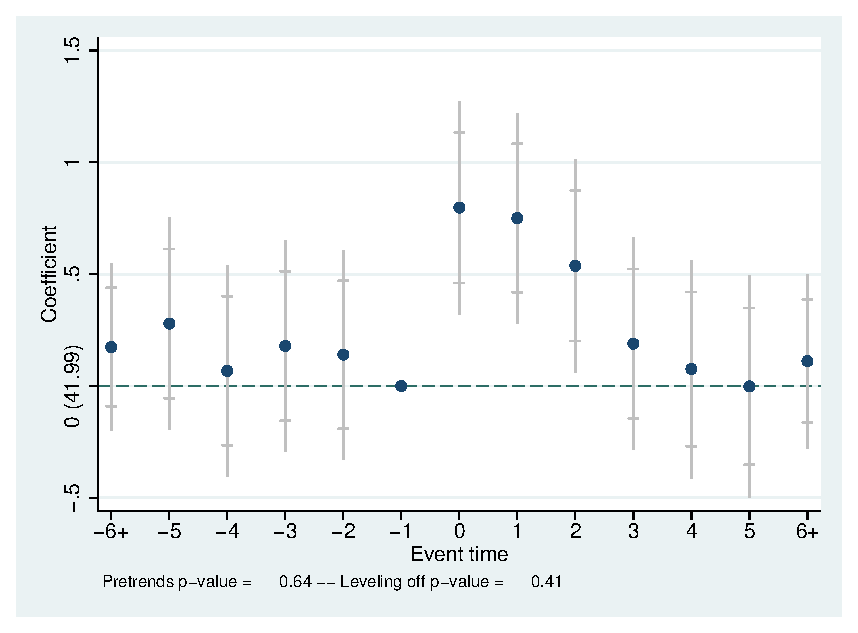
\includegraphics[width=0.9\linewidth]{../../output/analysis/plots/fhps_iv_outcome_plot}
  \caption{Event-study plot for outcome}
  \label{fig:overlayfhs1}
\end{subfigure}%
\begin{subfigure}{0.5\textwidth}
  \centering
  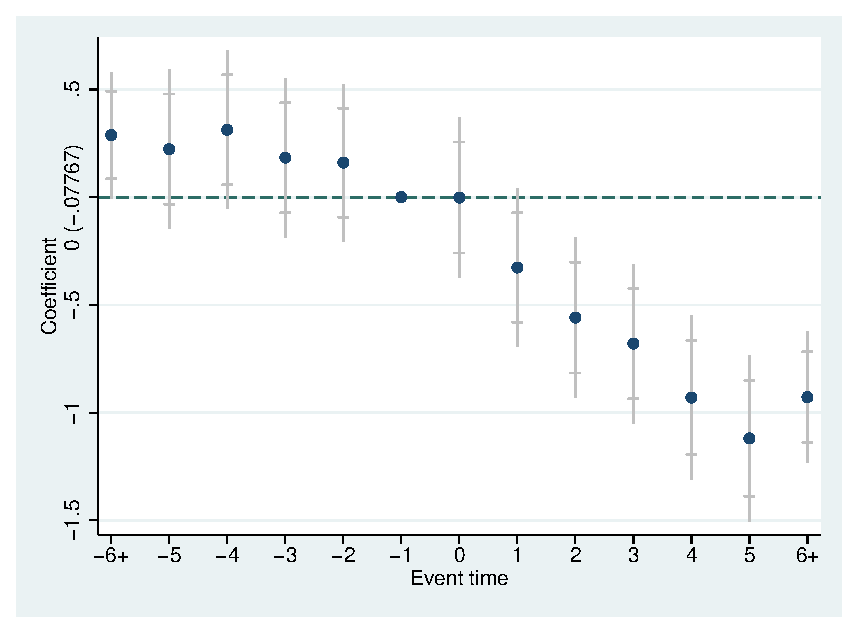
\includegraphics[width=0.9\linewidth]{../../output/analysis/plots/fhps_iv_proxy_plot}
  \caption{Event-study plot for proxy}
  \label{fig:overlayfhs2}
\end{subfigure}%

\begin{subfigure}{0.5\textwidth}
  \centering
  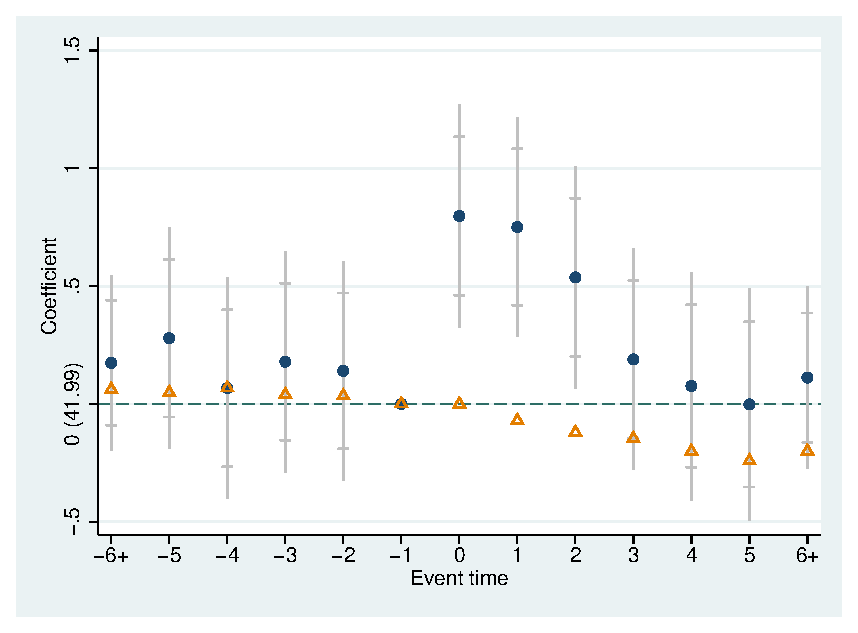
\includegraphics[width=0.9\linewidth]{../../output/analysis/plots/fhps_iv_proxy_outcome_plot}
  \caption{Align proxy to outcome}
  \label{fig:overlayfhs3}
\end{subfigure}%
\begin{subfigure}{0.5\textwidth}
  \centering
  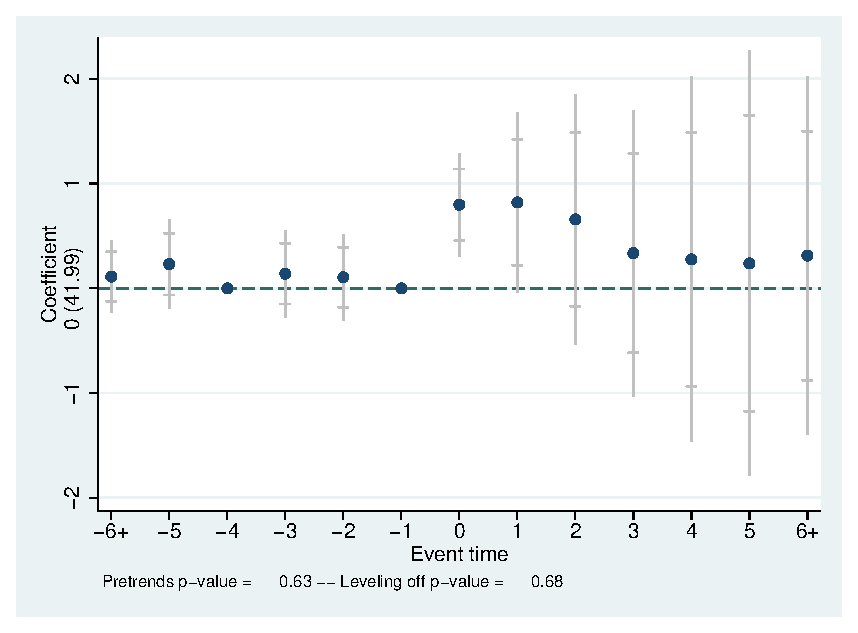
\includegraphics[width=0.9\linewidth]{../../output/analysis/plots/fhps_iv_subtraction_plot}
  \caption{Subtract rescaled confound from outcome}
  \label{fig:overlayfhs4}
\end{subfigure}%

\caption{Pre-trends adjustment using proxy variables for the confound following \cite{freyaldenhoven2019pre}}
\label{fig:overlayfhs}
\end{figure}


\subsubsection*{Estimation with heterogenous effects by cohort}

\begin{sloppypar}
\texttt{xtevent} allows estimation in settings with heterogeneous effects that vary by cohort using \citet{sun2021estimating}'s estimator through the \texttt{cohort} and \texttt{control\_cohort} options.
\end{sloppypar}
In the \texttt{cohort} option, the user must specify the variable that identifies the cohorts, and in the \texttt{control\_cohort} option, the variable that identifies the cohort that will be used as the control group.
In the following example, we first create the \texttt{time\_of\_treat} variable to identify the cohorts and then create the variable \texttt{last\_treat} to indicate the control group, which in this case are the last treated units.

\begin{stlog}
\input{../../output/analysis/plots/fhps_SA_estimation_modified.log.tex}\nullskip
\end{stlog}

The output is analogous to standard \xtevent output.
The estimated event-time path correspond to the weighted averages of event-study estimates comparing each treatment cohort to the control cohort.
\xtevent stores the estimates by cohort in the matrices \texttt{e(b\_interact)} and \texttt{e(V\_interact)}.

\subsubsection*{Least wiggly path of confounds consistent with the estimates}

\xteventplot allows for estimation and display of the least wiggly path of confound consistent with the estimates discussed in section \ref{sec:methods}, through the \texttt{smpath([type, subopt])}) option.
The default plot type is \texttt{line}.
With the additional suboptions \texttt{maxiter}, \texttt{technique}, \texttt{maxorder}, and \texttt{postwindow} we can control the optimization process, the maximum polynomial order for the confound path, and the number of post-event coefficients to include in the estimation of the path.

\begin{stlog}
\input{../../output/analysis/plots/fhps_smpath_modified.log.tex}\nullskip
\end{stlog}

In this case, the minimum polynomial order required to pass through the confidence region has order 4.
Figure \ref{fig:smpath} shows the resulting smoothest path.
If all of the dynamics of the estimated event-time path of the outcome variable are driven by an unmeasured confound, the jump at the time of the event implies that the confound would have to also jump at the time of the event.
Such confound path suggests that the estimated effects may be due to an effect of the policy, and not to a confound.

\begin{figure}[h!]
\begin{center}
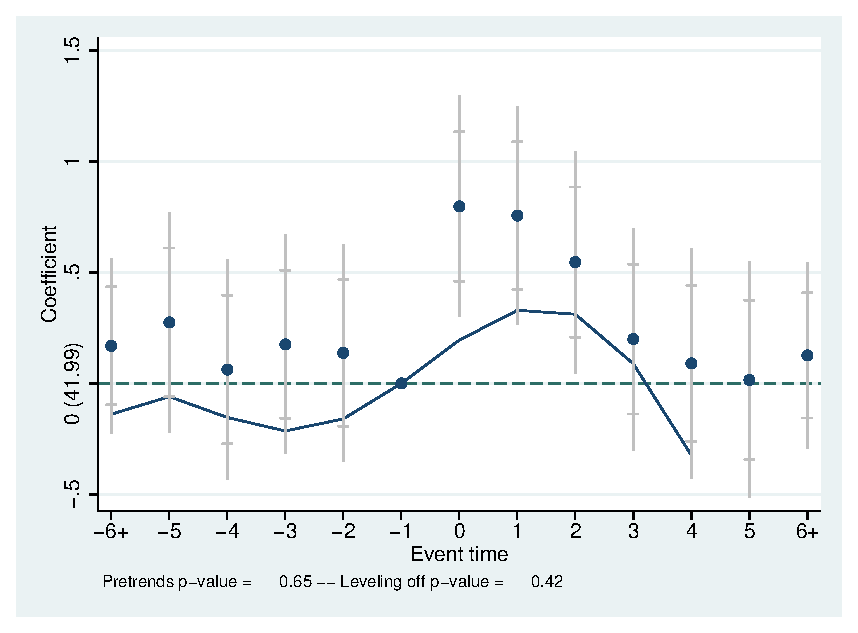
\epsfig{file=../../output/analysis/plots/fhps_smpath}
\end{center}
\caption{Least wiggly path through the confidence region}
\label{fig:smpath}
\end{figure}

%%%%%%%%%%%%%%% Empirical Application

\subsection{Empirical application}\label{sec:app}

\citet{martinez2022mobility} analyzes the effect of a tax reform in the Swiss canton of Obwalden in 2006.
The reform modified the income tax schedule providing tax rate reductions to high-income taxpayers.
We focus on her analysis of the reform's effect on Obwalden's tax revenue from wealth taxes.\footnote{See Figure 9 in \citet{martinez2022mobility}.}
She shows that the reform had a negative impact on the per-capita tax revenues of Obwalden's government.\footnote {\citet{martinez2022mobility} describes several mechanisms which would explain the negative impact on tax revenues.
For instance, while the reform was successful at attracting high-income taxpayers from other cantons, it decreased tax revenue from high-income taxpayers already living in Obwalden.}

The data is a balanced panel of 702 observations from 26 cantons from 1990 to 2016.
Only one canton --Obwalden-- is treated.\footnote{We obtained this subset from the replication files on Martinez's personal website at \href{https://sites.google.com/view/isabelzmartinez/publications}{https://sites.google.com/view/isabelzmartinez/publications} in April 2023.}
We estimate a modified version of equation \eqref{eq:event_study_plot}:

\begin{equation}\label{eq:martinez}
y_{it} = \sum_{k=-5,k\neq -1}^{9}\delta_k \Delta z_{i,t-k} + \delta_{10} z_{i,t-10} + \delta_{-6}(1-z_{i,t+6}) + \alpha_{i} + \gamma_{t} + \varepsilon_{it}.
\end{equation}

Here, $y_{it}$ is per-capita revenue from wealth taxes in canton $i$ and year $t$.
The outcome $y_{it}$ is normalized to 100 in 2005.
The variable $z$ --the policy variable-- is one for Obwalden on 2006 or after and zero otherwise.
The $\delta$s parameters are the coefficients of the leads and lags of the differenced policy variable, plus the coefficients of the two end-points.
We normalize $\delta_{-1} = 0$.
The parameters $\alpha_i$ and $\gamma_{t}$ represent canton and year fixed effects, respectively.
$\varepsilon_{it}$ is an error term.

We start by loading the dataset, specifying the unit and time variables, and displaying some values of the dependent and policy variables around the treatment year:

\begin{stlog}
\input{../../output/analysis/plots/martinez_load_data.log.tex}\nullskip
\end{stlog}

We now estimate equation \ref{eq:martinez} to capture the dynamic effects of the reform on tax revenues.
We use an estimation window of 5 pre-event periods, 9 post-event periods, and two endpoints.
To adjust for pretrends, we use a linear trend adjustment.
The unit and time variables do not need to be specified because the data was \texttt{xtset} previously.
With the option \texttt{reghdfe}, we can estimate this equation using the \texttt{reghdfe} command of \citet{Correia2017:HDFE}.
Using \texttt{reghdfe} enables two-way clustered standard errors through the \texttt{vce} option.
We also specify the imputation rule \texttt{stag} and add weights.\footnote{With this, our results match those in \citet{martinez2022mobility} (cf. Figure 9 in \citeauthor{martinez2022mobility} \citeyear{martinez2022mobility}).}

\begin{stlog}
\input{../../output/analysis/plots/martinez_pretrend.log.tex}\nullskip
\end{stlog}

We use \xteventplot to display an event-study graph.
\xtevent allows for several options to modify the graph's appearance.
We modify the graph to suppress the sup-t confidence intervals, the p-values from overidentification tests.
We also change the colors and add axis titles.

\begin{stlog}
\input{../../output/analysis/plots/martinez_plot.log.tex}\nullskip
\end{stlog}

\begin{figure}[h!]
\begin{center}
\includegraphics[width=0.9\textwidth]{../../output/analysis/plots/martinez_plot}
\end{center}
\caption{Dynamic effect of tax reform}
\label{fig:martinez_default}
\end{figure}

Figure \ref{fig:martinez_default} indicates that the introduction of the regressive tax reform in Obwalden decreased its government's tax revenues (measured per capita and relative to the level in 2005). The strongest decrease was nearly 58\% and came after 2 years of the reform.

\subsubsection*{Hypothesis tests}

We can use \texttt{xteventtest} to test for different hypotheses about the event-study coefficients after \texttt{xtevent}.
For instance, we repeat the estimation with standard errors clustered by canton and use the \texttt{coefs} option to test if the coefficients for event-times 0, 1, 2, and 3 are equal to zero jointly.

\begin{stlog}
\input{../../output/analysis/plots/martinez_test_coefs.log.tex}\nullskip
\end{stlog}
The test indicates that the effects are different from zero.
We can also test if the estimated policy effects are constant across time:

\begin{stlog}
\input{../../output/analysis/plots/martinez_constanteff.log.tex}\nullskip
\end{stlog}

This test suggests that the effects are not constant over time.
Last, we conduct an overidentification test to see if the effects are leveling off.
To do this, we ask \texttt{xteventtest} to use the last two post-event coefficients.

\begin{stlog}
\input{../../output/analysis/plots/martinez_overidpost.log.tex}\nullskip
\end{stlog}

In this case, the test suggests that the effects are not leveling off, and a model with additional post-event periods may be appropriate.

%%%%%%%%%%%%%% Section 5: conclusions %%%%%%%%%%%%%
%\section{Conclusions}
%Conclusions...

\section{Acknowledgements}
We are grateful to the many users of \texttt{xtevent} that have provided feedback. We acknowledge financial support from the National Science Foundation under Grant No. 1558636 (Hansen), from the SUPER RA Program at Harvard (Shapiro), and from Colombia Cient\'{i}fica – Alianza EFI \#60185 contract \#FP44842-220-2018, funded by The World Bank through the Scientific Ecosystems, managed by the Colombian Administrative Department of Science, Technology and Innovation (P\'{e}rez P\'{e}rez). The views expressed herein are those of the authors and do not necessarily reflect the views of the Federal Reserve Bank of Philadelphia, the Federal Reserve System, Banco de M\'exico, or the funding sources. 

\textcolor{red}{Simon added the above based on our last paper - please confirm/update.}
% discussion of the Stata Journal document class.
%\input sj.tex
% discussion of the Stata Press LaTeX package for Stata output.
%\input stata.tex

\bibliographystyle{sj}
\bibliography{sj}

\begin{aboutauthors}
Simon Freyaldenhoven is a Senior Machine Learning Economist at the Federal Reserve Bank of Philadelphia.

Christian B. Hansen is the Wallace W. Booth Professor of Econometrics and Statistics at the University of Chicago Booth School of Business.

Jorge P\'erez P\'erez is a Research Economist at Banco de México.

Jesse M. Shapiro is the George Gund Professor of Economics and Business Administration at Harvard University and a Research Associate at the National Bureau of Economic Research.

\end{aboutauthors}


\clearpage

\appendix

\section{Details about trend extrapolation}
\label{sec:app_trend}
Let $T_G \leq L_G$ be the number of periods prior to $G$ used estimate the trend parameters, and $T_M \leq M$ be the number of ``post-event'' periods where the trend is active.
We assume $f_k \neq 0$ for $k \in \left[-G-T_G,T_M \right]$ and $0$ otherwise.
We do not use any policy-affected periods, or endpoints, to estimate $\phi$.
We then have moments given by
\[
\widehat{\delta}_{k}-\phi'f_{k}=0
\]
for $k=-G-T_G,...,-G-1$. Let $\widehat{\delta}_{T_G}$ be the $T_{G}$-vector
collecting $\widehat{\delta}_{k}$. Let $H_{T_G}$ be the $T_{G}\times\dim\left(\phi\right)$
matrix whose $j^{th}$ row is $f_{k}^{'}$ for $k=j-1-G-T_{G}$.

A minimum distance estimator $\hat{\phi}$ of $\phi$ solves
\begin{align*}
\hat{\phi} & =\arg\min_{\phi}\hat{h}\left(\phi\right)'\hat{W}\hat{h}\left(\phi\right)\\
\hat{h}\left(\phi\right) & =\widehat{\delta}_{T_G}-H_{T_G}\phi.
\end{align*}
Solving the FOC gives
\[
\begin{array}{rl}
0 & =-H_{L}^{\prime}\widehat{W}(\widehat{\delta}_{T_G}-H_{L}\widehat{\phi})\\
\widehat{\phi} & =(H_{T_G}^{\prime}\widehat{W}H_{T_G})^{-1}H_{T_G}^{\prime}\widehat{W}\widehat{\delta}
\end{array}
\]

Under suitable regularity conditions we have that
\[
\sqrt{n}\left(\begin{array}{c}
\widehat{\phi}-\phi_{0}\\
\widehat{\delta}_{T_G}-\delta_{L0}
\end{array}\right)\to N\left(0,\begin{bmatrix}\Lambda_{T_G}\Omega_{T_G}\Lambda_{T_G}^{\prime} & \Lambda_{T_G}\Omega_{T_G}\\
\Omega_{T_G}\Lambda_{T_G}^{\prime} & \Omega_{T_G}
\end{bmatrix}\right)
\]
where
\[
\Lambda_{T_G}=(H_{T_G}^{\prime}WH_{T_G})^{-1}H_{T_G}^{\prime}W
\]
and $\Omega_{T_G}$ is the asymptotic variance of $\widehat{\delta}_{T_G}$.
The feasible efficient weighting matrix is $\widehat{W}=\widehat{\Omega}_{T_G}^{-1}\to\Omega_{T_G}^{-1}$,
and with $W=\Omega_{T_G}^{-1}$ we have that $\Lambda_{T_G}\Omega_{T_G}\Lambda_{T_G}^{\prime}=(H_{T_G}^{\prime}\Omega_{T_G}^{-1}H_{T_G})^{-1}.$

\subsection{Estimation and inference on adjusted event-time path}

Now let $\hat{\delta}$ be the vector containing the entire estimated
event-time path, so $\dim\left(\hat{\delta}\right)=\dim\left(\delta\right)=M+L_{M}+G+L_{G}+2$.
Let $H$ be the $\dim\left(\delta\right)\times\dim\left(\phi\right)$
matrix whose $j^{th}$ row is $f_{k}^{'}$ for $k=j-2-G-L_{G}$. Given
the estimate $\widehat{\phi}$ we obtain the plugin estimate $\hat{\delta}^{*}$
of the adjusted event-time path by
\[
\hat{\delta}^{*}=\widehat{\delta}-H\hat{\phi}.
\]
Let $\Lambda=\begin{bmatrix}\boldsymbol{0} & \Lambda_{T_G} & \boldsymbol{0}\end{bmatrix}$,
with $\boldsymbol{0}$ conformable matrices of 0s ($\dim\left(\phi\right)\times1$
and $\dim\left(\phi\right)\times\left(\dim\left(\delta\right)-L_{G}\right)$,
respectively), $\widehat{\Lambda}$ be its sample analogue, and $I$
be a $\dim\left(\delta\right)\times\dim\left(\delta\right)$ identity
matrix. Hence $\hat{\delta}^{*}=\widehat{\delta}-H\hat{\phi}=\left(I-H\widehat{\Lambda}\right)\widehat{\delta}$
and it follows that (again under suitable conditions)
\[
\sqrt{n}\left(\widehat{\delta}^{*}-\delta_{0}^{*}\right)\to N\left(0,\Omega-H\Lambda\Omega-\Omega\Lambda^{\prime}H^{\prime}+H\Lambda\Omega\Lambda^{\prime}H^{\prime}\right)
\]
where
\[
\delta_{0,k}^{*}=\begin{cases}
0, & k<-G\\
\sum_{m=-G}^{k}\beta_{m}, & -G\le k\le M\\
\sum_{m=-G}^{M}\beta_{m}, & k>M.
\end{cases}
\]
Hypothesis testing for pre-trends and for dynamics leveling off can
now proceed as in the TWFE case, replacing $\widehat{\delta}$ with
$\hat{\delta}^{*}$.

\subsection{Covariance of adjusted event-time path and coefficient on controls}

For some purposes we may be interested in testing hypotheses jointly on $\left(\delta_{0}^{*},\psi_{0}\right)$.
% Since $\widehat{\delta}$ and $\widehat{\psi}$ are estimated in the same regression. Therefore
% we should be able to compute $\widehat{V}$ a consistent estimator
% for $V$, where
% \begin{align*}
% \sqrt{n}\begin{pmatrix}\widehat{\delta}-\delta_{0}\\
% \widehat{\psi}-\psi_{0}
% \end{pmatrix}\to N(0,V)
% \end{align*}
Since $\widehat{\delta}^{*}=(I-H\widehat{\Lambda})\widehat{\delta}$, we have
\begin{align*}
\sqrt{n}\begin{pmatrix}\widehat{\delta}^{*}-\delta_{0}^{*}\\
\widehat{\psi}-\psi_{0}
\end{pmatrix}=\begin{pmatrix}I-H\widehat{\Lambda} & 0\\
0 & I
\end{pmatrix}\sqrt{n}\begin{pmatrix}\widehat{\delta}-\delta_{0}\\
\widehat{\psi}-\psi_{0}
\end{pmatrix}\to\begin{pmatrix}I-H\Lambda & 0\\
0 & I
\end{pmatrix}N(0,V),
\end{align*}
with $0$ conformable matrices of zeros ($\text{dim}(\delta)\times\text{dim}(\psi)$
for the upper right and $\text{dim}(\psi)\times\text{dim}(\delta)$
for the lower left) and $I$ conformable identity matrices ($\text{dim\ensuremath{\left(\delta\right)}}$
for the upper left and $\text{dim}\left(\psi\right)$ for the lower
right). Finally, let $\Omega_{\psi}$ denote the $\text{dim}(\psi)\times\text{dim}(\psi)$
asymptotic variance of $\widehat{\psi}$ and $\Omega_{\delta,\psi}$
denote the $\text{dim}(\psi)\times\text{dim}(\delta)$ asymptotic
covariance between $\widehat{\delta},\widehat{\psi}$. We can express
\begin{align*}
V & =\begin{pmatrix}\Omega & \Omega_{\delta,\psi}^{\prime}\\
\Omega_{\delta,\psi} & \Omega_{\psi}
\end{pmatrix}
\end{align*}
and the asymptotic variance of $\left(\hat{\delta}^{*},\hat{\psi}\right)$ is
\begin{align*}
\begin{pmatrix}I-H\Lambda & 0\\
0 & I
\end{pmatrix}\begin{pmatrix}\Omega & \Omega_{\delta,\psi}^{\prime}\\
\Omega_{\delta,\psi} & \Omega_{\psi}
\end{pmatrix}\begin{pmatrix}I-\Lambda^{\prime}H^{\prime} & 0\\
0 & I
\end{pmatrix}=\begin{pmatrix}(I-H\Lambda)\Omega(I-\Lambda^{\prime}H^{\prime}) & (I-H\Lambda)\Omega_{\delta,\psi}^{\prime}\\
\Omega_{\delta,\psi}(I-\Lambda^{\prime}H^{\prime}) & \Omega_{\psi}
\end{pmatrix}.
\end{align*}

\section{Details for Smoothest Path}
\label{sec:smoothest_path}

\subsection{The smoothest path proposal}

We denote the dimension of $\delta$ as $K \equiv G + M + L_G + L_M + 2$. For $v$ a finite-dimensional coefficient vector and $k$ an integer, define the polynomial term
\begin{align*}
\delta_k^*(v) = \sum_{j=1}^{\dim(v)} v_j (\frac{k-s_1}{s_2})^{j-1},
\end{align*}
 where $v_j$ denotes the $j^{\text{th}}$ element of coefficient vector $v$ and $\dim(v)$ denotes the dimension of this vector. $s_1$ and $s_2$ denote constants that shift and scale the event time (range of the polynomial). We set $s_1 = -G-L_G-1$ and $s_2 = M + L_M + G + L_G +2$. Let $\delta^*(v)$ collect the elements $\delta_k^*(v)$ for $-G-L_G-1 \leq k \leq M+L_M$, so that $\delta^*(v)$ reflects a polynomial path in event time with coefficients $v$.

\xtevent plots the least ``wiggly'' confound whose path is contained in the Wald region $CR(\delta)$ for the event-time path of the outcome. Specifically, it plots $\delta^*(v^*)$, where

\begin{align}
  p^* &= \min\{\dim(v): \delta^*(v) \in CR(\delta)\} \text{ and}  \label{eq:max_order} \\
  v^* &= \arg\min_{v}\{v_{p^*}^2: \dim(v)=p^*, \delta^*(v) \in CR(\delta)\}. \label{eq:min_coeff}
\end{align}

Intuitively, the Wald confidence region represents the set of event time paths for which a joint F-test of the observed point estimates is not rejected. Since this region is an ellipsis, there is no straightforward graphical illustration of this region in an event plot.

To plot the smoothest path we solve a two-part problem.  In \eqref{eq:max_order} we find the smallest order $p^*$ such that a polynomial of order $p^*$ is fully contained in the Wald region $CR(\delta)$. In \eqref{eq:min_coeff}, we then choose the polynomial with the lowest coefficient on the highest order term of that polynomial.

In practice we have a normalization of the event path, such that $\delta_{k} = 0$ for at least one $k$ (e.g. usually at $k=-1$). We will use $\mathcal{N}$ to denote the set of size $N$ that collects all normalized coefficients, such that $\delta_{k}^*(v)=0$ for $k \in \mathcal{N}$. Throughout we only consider the case $N\in\{1,2\}$, i.e. we allow for at most two normalizations.

\subsection{Implementation}

\subsubsection{Finding $p^*$}

We start with the problem of finding $p^*$ in \eqref{eq:max_order}. We define $\Sigma$ as the covariance matrix of $\hat \delta$ with added zeros in the rows and columns corresponding to the normalized coefficients.

Since $p^*$ is generally small, it is feasible to solve \eqref{eq:max_order} iteratively as follows:
\begin{algorithm}
\caption{Finding $p^*$}
\label{alg:find_p}
\begin{algorithmic}
\State $p^* \gets 0$
\State feasible $\gets$ 0
\While {feasible = 0}
    \State $p^* \gets p^*+1$
  \State feasible $\gets$ SolutionInWaldRegion($\hat\delta,p^*,\alpha$)
\EndWhile
\end{algorithmic}
\end{algorithm}

\begin{algorithm*}
\begin{algorithmic}
\Function{SolutionInWaldRegion}{$\hat\delta,p^*,\alpha$}
\State $W^*=\min_{v:dim(v)=p^*} [\delta^*(v)-\hat{\delta}]'\Sigma^{-1}[\delta^*(v)-\hat{\delta}] \; \text{s.t. } \delta_{k_n}^*(v)=0 \text{ for } n \in \mathcal{N}$
\Comment $\Sigma^{-1}$ denotes the generalized inverse.
\State \textbf{return} $\textbf{1}(W^* \le c^{1-\alpha})$
\Comment $c^{1-\alpha}$ is the $1-\alpha$ quantile of a $\chi^2$ random variable with $(K-N)$ degrees of freedom.
\EndFunction
\end{algorithmic}
\end{algorithm*}
%\begin{remark}
Note that $p^*$ is less than $K=dim(\delta)$ by construction and thus the loop in Algorithm \ref{alg:find_p} is (at least theoretically) guaranteed to converge after at most $K$ rounds. To ensure numerical stability, we restrict $p^*$ to be less than or equal to ten in our implementation (with a user-option to reduce the upper bound further). If $p^{*}>10$, we conclude ``no smooth path exists".
%\end{remark}

To find $W^*$ in practice, we use the first order conditions of the minimization of the Wald statistic subject to the constraints on the normalized coefficients.

To do this we write the smoothest path polynomial in matrix notation as $\delta^*(v) = \underset{K\times p^*}{F} \underset{p^* \times 1}{v} $, where $F_{kj} = \left(\frac{k-s_1}{s_2}\right)^{j-1}$ for $k=1, \ldots, K$. The rows of $F$ collect the polynomial terms for a given (shifted) event time $k$, and the vector $v$ collects the polynomial coefficients. The problem for finding $W^*$ can be rewritten as:
\begin{align}
\min_v \left[Fv-\hat{\delta}\right]'\Sigma^{-1}\left[Fv-\hat{\delta}\right] \text{s.t. } \delta_{k}^*(v)=0 \text{ for } k \in \mathcal{N}. \label{eq:optimization_W*}
\end{align}

From the Lagrangian, the first order conditions are:
\begin{align*}
F'\Sigma^{-1}F v &=  F' \Sigma^{-1} \hat{\delta} +\frac{1}{2} \lambda A_{norm}'\\
A_{norm} v &= 0
\end{align*}

Here, $A_{norm}$ is the matrix with the rows of $F$ that correspond to the normalized coefficients. Algebra then shows that $v(\lambda)=(F'\Sigma^{-1}F)^{-1}[F' \Sigma^{-1} \hat{\delta} + \frac{1}{2} \lambda A_{norm}']$, and plugging this back into the second first order condition above yields

\begin{equation*}
\lambda = -2[A_{norm}(F'\Sigma^{-1}F)^{-1}A_{norm}']^{-1}A_{norm}(F'\Sigma^{-1}F)^{-1} F' \Sigma^{-1} \hat{\delta}.
\end{equation*}

Thus, the solution for $v$ is given by
\begin{align*}
\tilde v= (F'\Sigma^{-1}F)^{-1} \left[ F' \Sigma^{-1} \hat{\delta} - A_{norm}'[A_{norm}(F'\Sigma^{-1}F)^{-1}A_{norm}']^{-1}A_{norm} (F'\Sigma^{-1}F)^{-1}F' \Sigma^{-1} \hat{\delta}\right].
\end{align*}

We can write the solution for $v$ as a matrix product. Let $XX \equiv \begin{bmatrix} 2F'\Sigma^{-1}F & A_{norm}' \\ A_{norm} & \underset{N \times N} {\mathbf{0}} \end{bmatrix} $ and $Xy \equiv \begin{bmatrix} 2F'\Sigma^{-1}\hat{\delta} \\ \underset{N \times N}{\mathbf{0}} \end{bmatrix} $. Then the solution for $v$ is the vector with the first $K$ rows of $\Tilde{v} = (XX)^{-1} Xy$.

\subsubsection{Finding the optimal path given $p^*$}


Once we we have found a solution to \eqref{eq:max_order} using Algorithm \ref{alg:find_p}, the next step is to find the polynomial with the lowest coefficient on the $p^*$ term that is still contained in the Wald region (see equation \ref{eq:min_coeff}). First note that by construction $v^2_{p^*} \ne 0$ (If not, Algorithm \ref{alg:find_p} would have found a solution at $p^*-1$). $v^*$ can then be found through a simple constrained minimization on the vector $v$ (of dimension $p^*$):
\begin{align}
v^* &= \arg\min_{v} v_{p^*}^2 \label{eq:obj}\\
\text{such that }  & [\delta^*(v)-\hat{\delta}]\Sigma^{-1}[\delta^*(v)-\hat{\delta}] \le c^{1-\alpha}\} \label{eq:cons1}\\
\text{and } & \delta_{k}^*(v)=0 \text{ for } k \in \mathcal{N}, \label{eq:cons2}
\end{align}
with $\Sigma$ and $c^{1-\alpha}$ defined as above.

First, if $p^* \le N$, the constraint in \eqref{eq:cons2} implies that $v^*=0$ and we are done.
Next, if $p^*>N$, we note that $v^*$ will always be on the boundary of the Wald region. Thus, the constraint in \eqref{eq:cons1} will always be binding, and we can substitute both constraints directly to solve for $v^*$. In particular, given a set $\mathcal{N}$ of normalized coefficients and the constraint in \eqref{eq:cons1}, we can solve for some of the other coefficients. If $p^*>N+1$, we use an unconstrained optimization to solve for the remaining ones after that.

Specifically, partition the matrices $A_{norm}$ and $F$ into three parts as follows
\begin{align*}
A_{norm} &= [ \underset{N \times (p^* - N - 1)}{A_b}, \underset{N \times N}{A_1}, \underset{N \times 1}{A_2}] \\
F &= [\underset{K \times  (p^* - N -1) }{F_b},\underset{K \times N }{F_1},\underset{K \times 1}{F_2}],
\end{align*}
with the vector $v$ partioned accordingly into $v=[v_b; v_1; v_2]$.
We will solve for the coefficients $v_1$ and $v_2$ using the constraints in \eqref{eq:cons2} and \eqref{eq:cons1} respectively, and then solve for the coefficients $v_b$ by unconstrained minimization. To do so, first note that, because $A_{norm}$ contains the rows of $F$ associated with the normalized coefficients,
\begin{align}
A_{norm}v =  A_b v_b + A_1 v_1 + A_2 v_2 = 0 \;\text{and thus }v_1 = {A_1}^{-1}(- A_b v_b - A_2 v_2).\label{eq:def_v1}
\end{align}
It follows that
\begin{align*}
\delta^*(v)= Fv = F_b v_b + F_1 v_1 + F_2 v_2 = F_b v_b - F_1 \big[ {A_1}^{-1}( A_b v_b + A_2 v_2)\big] + F_2 v_2,
\end{align*}
and the constraint in \eqref{eq:cons1} becomes

\begin{align*}
&\bigg[(F_b - F_1 {A_1}^{-1}A_b) v_b - \hat{\delta} + (F_2 - F_1 {A_1}^{-1} A_2) v_2 \bigg]' \Sigma ^ {-1}\bigg[(F_b - F_1 {A_1}^{-1} A_b) v_b - \hat{\delta} + (F_2 - F_1 {A_1}^{-1}A_2) v_2  \bigg] \\\nonumber
&= c^{1 - \alpha}.
\end{align*}

Expanding this yields
\begin{align*}
0 = &\bigg([(F_b - F_1 {A_1}^{-1}A_b) v_b - \hat{\delta}]' \Sigma ^ {-1} [(F_b - F_1 {A_1}^{-1}A_b) v_b - \hat{\delta}] - c^{1 - \alpha} \bigg) \\
&\qquad + 2 \bigg([(F_b - F_1 {A_1}^{-1}A_b) v_b - \hat{\delta}]' \Sigma ^ {-1} [(F_2 - F_1 {A_1}^{-1} A_2) \bigg) v_2 \nonumber \\
&\qquad +  v_2'\bigg([(F_2 - F_1 {A_1}^{-1} A_2)]'\Sigma ^ {-1} [(F_2 - F_1 {A_1}^{-1}A_2)] \bigg)v_2 .
\end{align*}

This is a quadratic expression for (the scalar) $v_2$ in terms of $v_b$ and, defining the scalars $d_0$, $d_1$ and $d_2$ as

\begin{align*}
d_0 &= \big[(F_2 - F_1 {A_1}^{-1} A_2)\big]'\Sigma ^ {-1} \big[(F_2 - F_1 {A_1}^{-1}A_2)\big], \\
d_1(v_b) &= 2 \bigg([(F_b - F_1 {A_1}^{-1}A_b) v_b - \hat{\delta}]' \Sigma ^ {-1} [(F_2 - F_1 {A_1}^{-1} A_2) \bigg), \text{and} \\
d_2(v_b) &= \bigg([(F_b - F_1 {A_1}^{-1}A_b) v_b - \hat{\delta}]' \Sigma ^ {-1} [(F_b - F_1 {A_1}^{-1}A_b) v_b - \hat{\delta}] - c^{1 - \alpha} \bigg)
\end{align*}

simplifies to $d_0 v_2^2 +  d_1(v_b) v_2 + d_2 (v_b)=0$.

Using the quadratic formula, we can then solve for $v_2$ by solving the minimization problem.
\begin{align}
\label{eq:quad_solution}
    v_2(v_b) = \dfrac{-d_1(v_b) \pm \sqrt{d_1(v_b)^2 - 4 d_0 d_2(v_b)}}{2 d_0}.
\end{align}
Note that, by definition, $v_2 = v_{p^*}$.

Further, if $p^*= N+1$, $v_b$ is empty and thus $v_2$ does not depend on $v_b$. \eqref{eq:quad_solution} results in two solutions, $v_2^+$ and $v_1^-$, corresponding to the sign ambiguity in \eqref{eq:quad_solution}. We choose the solution $v^*_2$ with the smaller absolute value.

If $p^*> N+1$, the constrained optimization in \eqref{eq:obj}-\eqref{eq:cons2} is equivalent to the following:
\begin{align}
  v^2_2 =  \min_{v_b} \min_{\{+,-\}} \bigg( \dfrac{-d_1(v_b) \pm \sqrt{d_1(v_b)^2 - 4 d_0 d_2(v_b)}}{2 d_0} \bigg)^2,\label{eq:quad_solution_min}
\end{align}
where the inner minimization is over the sign in the quadratic formula.

At this point we have both $v^*_2$ and $v^*_b$. Recovering $v^*_1$ using \eqref{eq:def_v1}, we obtain $v^*=[v^*_b, v^*_1,  v^*_2]$.

% \section{Imputation of missing policy variable values}
% \label{sec:imputation}

\section{Policy variable imputation}
\label{sec:impute}

\xtevent allows for different imputations of policy variable values under different policy adoption schemes, through the \texttt{impute(type)} option.

To illustrate this option, we use the simulated data example of section \ref{sec:examples} and show how the imputation works on the event-time dummies under the \texttt{stag} imputation scheme. For the example, we add some missing values to unit 19. Then, we differentiate the policy variable. \texttt{xtevent} uses leads and lags of the differentiated policy variable to generate the event-time dummies, following equation \eqref{eq:event_study_plot}. We ask \texttt{xtevent} to generate the event-time dummies without any imputation and specify the option \texttt{savek(stub, noestimate)} to save them without estimating the model.

\begin{stlog}
	. replace z=. if id==2 \& t<3
(2 real changes made, 2 to missing)
{\smallskip}
. qui xtevent y_jump_m x_jump_m, panelvar(id) timevar(t) policyvar(z) ///
>  window(5) savek(v, noestimate)
{\smallskip}
\nullskip
\end{stlog}

The event-time dummies with the subfix \texttt{m\#} correspond to leads of the differentiated policy variable, as described in section \ref{sec:package}. Now we display these event-time dummies for unit 19 in some periods. Notice that the event-time dummies have missing values because we are assuming nothing about the policy variable outside the observed time range.

\begin{stlog}
	. list id t z v_eq_m6 -v_eq_m1 if inlist(id,1,2) \& (t<=10 | t>=31), ///
> separator(10) noobs
{\smallskip}
  {\TLC}\HLI{73}{\TRC}
  {\VBAR} id    t   z   v_eq_m6   v_eq_m5   v_eq_m4   v_eq_m3   v_eq_m2   v_eq_m1 {\VBAR}
  {\LFTT}\HLI{73}{\RGTT}
  {\VBAR}  1    1   0         1         0         0         0         0         0 {\VBAR}
  {\VBAR}  1    2   0         1         0         0         0         0         0 {\VBAR}
  {\VBAR}  1    3   0         1         0         0         0         0         0 {\VBAR}
  {\VBAR}  1    4   0         1         0         0         0         0         0 {\VBAR}
  {\VBAR}  1    5   0         1         0         0         0         0         0 {\VBAR}
  {\VBAR}  1    6   0         1         0         0         0         0         0 {\VBAR}
  {\VBAR}  1    7   0         1         0         0         0         0         0 {\VBAR}
  {\VBAR}  1    8   0         1         0         0         0         0         0 {\VBAR}
  {\VBAR}  1    9   0         1         0         0         0         0         0 {\VBAR}
  {\VBAR}  1   10   0         1         0         0         0         0         0 {\VBAR}
  {\LFTT}\HLI{73}{\RGTT}
  {\VBAR}  1   31   0         0         0         0         0         0         1 {\VBAR}
  {\VBAR}  1   32   1         0         0         0         0         0         0 {\VBAR}
  {\VBAR}  1   33   1         0         0         0         0         0         0 {\VBAR}
  {\VBAR}  1   34   1         0         0         0         0         0         0 {\VBAR}
  {\VBAR}  1   35   1         0         0         0         0         0         0 {\VBAR}
  {\VBAR}  1   36   1         .         .         0         0         0         0 {\VBAR}
  {\VBAR}  1   37   1         .         .         .         0         0         0 {\VBAR}
  {\VBAR}  1   38   1         .         .         .         .         0         0 {\VBAR}
  {\VBAR}  1   39   1         .         .         .         .         .         0 {\VBAR}
  {\VBAR}  1   40   1         .         .         .         .         .         . {\VBAR}
  {\LFTT}\HLI{73}{\RGTT}
  {\VBAR}  2    1   .         .         .         .         .         .         . {\VBAR}
  {\VBAR}  2    2   .         .         .         .         .         .         . {\VBAR}
  {\VBAR}  2    3   0         0         0         0         0         0         1 {\VBAR}
  {\VBAR}  2    4   1         0         0         0         0         0         0 {\VBAR}
  {\VBAR}  2    5   1         0         0         0         0         0         0 {\VBAR}
  {\VBAR}  2    6   1         0         0         0         0         0         0 {\VBAR}
  {\VBAR}  2    7   1         0         0         0         0         0         0 {\VBAR}
  {\VBAR}  2    8   1         0         0         0         0         0         0 {\VBAR}
  {\VBAR}  2    9   1         0         0         0         0         0         0 {\VBAR}
  {\VBAR}  2   10   1         0         0         0         0         0         0 {\VBAR}
  {\LFTT}\HLI{73}{\RGTT}
  {\VBAR}  2   31   1         0         0         0         0         0         0 {\VBAR}
  {\VBAR}  2   32   1         0         0         0         0         0         0 {\VBAR}
  {\VBAR}  2   33   1         0         0         0         0         0         0 {\VBAR}
  {\VBAR}  2   34   1         0         0         0         0         0         0 {\VBAR}
  {\VBAR}  2   35   1         0         0         0         0         0         0 {\VBAR}
  {\VBAR}  2   36   1         .         .         0         0         0         0 {\VBAR}
  {\VBAR}  2   37   1         .         .         .         0         0         0 {\VBAR}
  {\VBAR}  2   38   1         .         .         .         .         0         0 {\VBAR}
  {\VBAR}  2   39   1         .         .         .         .         .         0 {\VBAR}
  {\VBAR}  2   40   1         .         .         .         .         .         . {\VBAR}
  {\BLC}\HLI{73}{\BRC}
\nullskip
\end{stlog}

We can generate the event-time dummies and endpoints after indicating \texttt{xtevent} to impute the policy variable by the \texttt{impute(type)} option, using as imputation rule \texttt{stag}. This imputation type first will verify that the policy variable follows staggered adoption. If so, \xtevent will impute the policy variable outside the observed values. Then, it will use the imputed policy variable to generate the event-time dummies and endpoints. We add the suboption \texttt{saveimp} to save the imputed policy variable as \texttt{z\_imputed}. We also differentiate the new imputed policy variable to see how its leads translate to the new event-time dummies.

\begin{stlog}
	. cap drop v*
{\smallskip}
. qui xtevent y_jump_m x_jump_m, panelvar(id) timevar(t) policyvar(z) ///
> window(5) savek(v, noestimate) impute(stag, saveimp) 
{\smallskip}
\nullskip
\end{stlog}

Now we can compare the imputed policy variable, its differentiated variable, and the event-time dummies and endpoints generated using the imputed policy variable. First, we can see that the policy variable has been imputed in the observed time range. Nonetheless, the imputation also implies that the policy variable follows a similar pattern outside the observed time range. When translating this to the event-time dummies, we can see imputed values for periods that would fall outside the observed time range.

\begin{stlog}
	. list id t z z_imputed v_eq_m6 -v_eq_m1 if inlist(id,1,2) \& (t<=10 | t>=31), ///
> separator(10) noobs abbreviate(6)
{\smallskip}
  {\TLC}\HLI{76}{\TRC}
  {\VBAR} id    t   z   z_im{\tytilde}d   v_e{\tytilde}m6   v_e{\tytilde}m5   v_e{\tytilde}m4   v_e{\tytilde}m3   v_e{\tytilde}m2   v_e{\tytilde}m1 {\VBAR}
  {\LFTT}\HLI{76}{\RGTT}
  {\VBAR}  1    1   0        0        1        0        0        0        0        0 {\VBAR}
  {\VBAR}  1    2   0        0        1        0        0        0        0        0 {\VBAR}
  {\VBAR}  1    3   0        0        1        0        0        0        0        0 {\VBAR}
  {\VBAR}  1    4   0        0        1        0        0        0        0        0 {\VBAR}
  {\VBAR}  1    5   0        0        1        0        0        0        0        0 {\VBAR}
  {\VBAR}  1    6   0        0        1        0        0        0        0        0 {\VBAR}
  {\VBAR}  1    7   0        0        1        0        0        0        0        0 {\VBAR}
  {\VBAR}  1    8   0        0        1        0        0        0        0        0 {\VBAR}
  {\VBAR}  1    9   0        0        1        0        0        0        0        0 {\VBAR}
  {\VBAR}  1   10   0        0        1        0        0        0        0        0 {\VBAR}
  {\LFTT}\HLI{76}{\RGTT}
  {\VBAR}  1   31   0        0        0        0        0        0        0        1 {\VBAR}
  {\VBAR}  1   32   1        1        0        0        0        0        0        0 {\VBAR}
  {\VBAR}  1   33   1        1        0        0        0        0        0        0 {\VBAR}
  {\VBAR}  1   34   1        1        0        0        0        0        0        0 {\VBAR}
  {\VBAR}  1   35   1        1        0        0        0        0        0        0 {\VBAR}
  {\VBAR}  1   36   1        1        0        0        0        0        0        0 {\VBAR}
  {\VBAR}  1   37   1        1        0        0        0        0        0        0 {\VBAR}
  {\VBAR}  1   38   1        1        0        0        0        0        0        0 {\VBAR}
  {\VBAR}  1   39   1        1        0        0        0        0        0        0 {\VBAR}
  {\VBAR}  1   40   1        1        0        0        0        0        0        0 {\VBAR}
  {\LFTT}\HLI{76}{\RGTT}
  {\VBAR}  2    1   .        0        0        0        0        1        0        0 {\VBAR}
  {\VBAR}  2    2   .        0        0        0        0        0        1        0 {\VBAR}
  {\VBAR}  2    3   0        0        0        0        0        0        0        1 {\VBAR}
  {\VBAR}  2    4   1        1        0        0        0        0        0        0 {\VBAR}
  {\VBAR}  2    5   1        1        0        0        0        0        0        0 {\VBAR}
  {\VBAR}  2    6   1        1        0        0        0        0        0        0 {\VBAR}
  {\VBAR}  2    7   1        1        0        0        0        0        0        0 {\VBAR}
  {\VBAR}  2    8   1        1        0        0        0        0        0        0 {\VBAR}
  {\VBAR}  2    9   1        1        0        0        0        0        0        0 {\VBAR}
  {\VBAR}  2   10   1        1        0        0        0        0        0        0 {\VBAR}
  {\LFTT}\HLI{76}{\RGTT}
  {\VBAR}  2   31   1        1        0        0        0        0        0        0 {\VBAR}
  {\VBAR}  2   32   1        1        0        0        0        0        0        0 {\VBAR}
  {\VBAR}  2   33   1        1        0        0        0        0        0        0 {\VBAR}
  {\VBAR}  2   34   1        1        0        0        0        0        0        0 {\VBAR}
  {\VBAR}  2   35   1        1        0        0        0        0        0        0 {\VBAR}
  {\VBAR}  2   36   1        1        0        0        0        0        0        0 {\VBAR}
  {\VBAR}  2   37   1        1        0        0        0        0        0        0 {\VBAR}
  {\VBAR}  2   38   1        1        0        0        0        0        0        0 {\VBAR}
  {\VBAR}  2   39   1        1        0        0        0        0        0        0 {\VBAR}
  {\VBAR}  2   40   1        1        0        0        0        0        0        0 {\VBAR}
  {\BLC}\HLI{76}{\BRC}
\nullskip
\end{stlog}


\section{Estimation in repeated cross-sectional datasets.}

\texttt{xtevent} allows estimation with repeated cross-sectional datasets when \texttt{policyvar} varies at the group level, and \texttt{panelvar} identifies the groups.
For instance, \texttt{panelvar} could indicate states at which \texttt{policyvar} changes, while the observations in the dataset should be individuals in each state. 
\texttt{xtevent} allow estimations in these settings directly with the \texttt{repeatedcs} option.
It also allows the two step procedure described in \citet{hansen2007generalized}.
To use the latter method, the user should first use the \texttt{get\_unit\_time\_effects} command to estimate unit-time effects and then use these estimations as input for \texttt{xtevent}.

We illustrate the use of \texttt{get\_unit\_time\_effects}.
First, we create a variable \texttt{state} that represents groups in which individuals receive the treatment in the same period.
Then, we call \texttt{get\_unit\_time\_effects}.
It saves\texttt{dta} file with the unit-time effects.

\begin{stlog}
. gen state=eventtime
{\smallskip}
. xtset, clear
{\smallskip}
. get_unit_time_effects y_jump_m x_jump_m, panelvar(state) timevar(t) ///
> saving("effect_file.dta", replace)
{\smallskip}
Linear regression, absorbing indicators         Number of obs     =      2,000
Absorbed variable: {\bftt{unittimeinteraction}}          No. of categories =      1,080
                                                F(   1,    919)   =       0.59
                                                Prob > F          =     0.4415
                                                R-squared         =     0.5447
                                                Adj R-squared     =     0.0096
                                                Root MSE          =     0.7332
{\smallskip}
\HLI{13}{\TOPT}\HLI{64}
    y_jump_m {\VBAR}      Coef.   Std. Err.      t    P>|t|     [95\% Conf. Interval]
\HLI{13}{\PLUS}\HLI{64}
    x_jump_m {\VBAR}   .0333291   .0432894     0.77   0.442    -.0516284    .1182867
       _cons {\VBAR}   42.16666   .0219049  1924.99   0.000     42.12367    42.20965
\HLI{13}{\BOTT}\HLI{64}
F test of absorbed indicators: F(1079, 919) = 1.013           Prob > F = 0.420
file effect_file.dta saved
\nullskip
\end{stlog}

Then, we keep one observation per state-time in the repeated cross-sectional data and merge the dataset with the unit-time effects.
Afterwards, we execute \texttt{xtevent}.
Since we end up using a smaller dataset for the estimation of the event-study, therefore this method can be faster than using the \texttt{repeatedcs} option.

\begin{stlog}
. qui bysort state t (z): keep if _n==1
{\smallskip}
. keep state t z
{\smallskip}
. qui merge m:1 state t using effect_file.dta, nogen
{\smallskip}
. xtevent _unittimeeffects, panelvar(state) timevar(t) policyvar(z) window(5)
{\smallskip}
No proxy or instruments provided. Implementing OLS estimator
{\smallskip}
Linear regression, absorbing indicators         Number of obs     =        783
Absorbed variable: {\bftt{state}}                        No. of categories =         27
                                                F(  40,    716)   =       2.09
                                                Prob > F          =     0.0001
                                                R-squared         =     0.1271
                                                Adj R-squared     =     0.0466
                                                Root MSE          =     0.5971
{\smallskip}
\HLI{13}{\TOPT}\HLI{64}
_unittimee{\tytilde}s {\VBAR}      Coef.   Std. Err.      t    P>|t|     [95\% Conf. Interval]
\HLI{13}{\PLUS}\HLI{64}
    _k_eq_m6 {\VBAR}    .125193   .1496943     0.84   0.403    -.1686992    .4190852
    _k_eq_m5 {\VBAR}   .3059997   .1907151     1.60   0.109    -.0684281    .6804274
    _k_eq_m4 {\VBAR}   -.067457   .1908708    -0.35   0.724    -.4421903    .3072764
    _k_eq_m3 {\VBAR}   .1560674   .1901574     0.82   0.412    -.2172653    .5294002
    _k_eq_m2 {\VBAR}   .0130564   .1879353     0.07   0.945    -.3559138    .3820265
    _k_eq_p0 {\VBAR}   .7827579   .1879387     4.16   0.000     .4137811    1.151735
    _k_eq_p1 {\VBAR}   .7056503   .1880443     3.75   0.000     .3364663    1.074834
    _k_eq_p2 {\VBAR}    .504723   .1885717     2.68   0.008     .1345035    .8749425
    _k_eq_p3 {\VBAR}    .252473   .1888205     1.34   0.182     -.118235     .623181
    _k_eq_p4 {\VBAR}   .1564468   .1914578     0.82   0.414    -.2194389    .5323325
    _k_eq_p5 {\VBAR}  -.1234141   .1943722    -0.63   0.526    -.5050216    .2581934
    _k_eq_p6 {\VBAR}   .1234968   .1534966     0.80   0.421    -.1778604    .4248541
             {\VBAR}
           t {\VBAR}
          8  {\VBAR}   .0543377   .1628964     0.33   0.739    -.2654739    .3741494
          9  {\VBAR}  -.0164568   .1631952    -0.10   0.920    -.3368551    .3039415
         10  {\VBAR}  -.1643727   .1632338    -1.01   0.314    -.4848469    .1561015
         11  {\VBAR}   .1225894   .1635376     0.75   0.454    -.1984811    .4436599
         12  {\VBAR}  -.0597104   .1636926    -0.36   0.715    -.3810852    .2616644
         13  {\VBAR}   .1498693   .1641559     0.91   0.362    -.1724152    .4721537
         14  {\VBAR}   .1020897   .1644289     0.62   0.535    -.2207307      .42491
         15  {\VBAR}   .0076888   .1648757     0.05   0.963    -.3160088    .3313863
         16  {\VBAR}     .13305   .1654226     0.80   0.421    -.1917214    .4578214
         17  {\VBAR}   .1533201   .1661387     0.92   0.356    -.1728572    .4794974
         18  {\VBAR}   .0228054   .1666432     0.14   0.891    -.3043623    .3499731
         19  {\VBAR}   .1024023   .1673021     0.61   0.541    -.2260589    .4308635
         20  {\VBAR}    .095213   .1683293     0.57   0.572    -.2352649     .425691
         21  {\VBAR}  -.0676372   .1689222    -0.40   0.689    -.3992793    .2640049
         22  {\VBAR}    .028276    .170072     0.17   0.868    -.3056234    .3621755
         23  {\VBAR}   .0151071   .1707856     0.09   0.930    -.3201933    .3504076
         24  {\VBAR}   .1357412   .1722658     0.79   0.431    -.2024653    .4739477
         25  {\VBAR}   .0136833   .1724831     0.08   0.937    -.3249498    .3523163
         26  {\VBAR}   .0662005   .1740932     0.38   0.704    -.2755937    .4079947
         27  {\VBAR}  -.0310915   .1757825    -0.18   0.860    -.3762023    .3140192
         28  {\VBAR}  -.0908547   .1772881    -0.51   0.608    -.4389213    .2572119
         29  {\VBAR}  -.1309403   .1788865    -0.73   0.464    -.4821451    .2202646
         30  {\VBAR}  -.1104622   .1801272    -0.61   0.540    -.4641029    .2431785
         31  {\VBAR}  -.1936314   .1812331    -1.07   0.286    -.5494431    .1621803
         32  {\VBAR}  -.0770778   .1825493    -0.42   0.673    -.4354737    .2813182
         33  {\VBAR}  -.0032709   .1838613    -0.02   0.986    -.3642427    .3577008
         34  {\VBAR}  -.1390926   .1857682    -0.75   0.454     -.503808    .2256229
         35  {\VBAR}  -.2293227   .1869708    -1.23   0.220    -.5963992    .1377538
             {\VBAR}
       _cons {\VBAR}  -.1442377   .1832237    -0.79   0.431    -.5039576    .2154822
\HLI{13}{\BOTT}\HLI{64}
F test of absorbed indicators: F(26, 716) = 0.665             Prob > F = 0.897
{\smallskip}
\nullskip
\end{stlog}


\end{document}
% END: main.tex


